% THIS IS AN EXAMPLE DOCUMENT FOR VLDB 2010
% based on ACM SIGPROC-SP.TEX VERSION 2.7
% Modified by  Gerald Weber <gerald@cs.auckland.ac.nz>


% This example *does* use the .bib file (from which the .bbl file
% is produced). REMEMBER HOWEVER: After having produced the .bbl file,
% and prior to final submission, you need to 'insert'  your .bbl file into
% your source .tex file so as to provide ONE 'self-contained' source file.

\documentclass[a4paper,12pt,oneside,titlepage]{book}
\renewcommand{\baselinestretch}{1.5}

%==============================================================
\usepackage[BoldFont, SlantFont, CJKchecksingle]{xeCJK}
\setCJKmainfont[Mapping=tex-text]{STSongti-TC-Light}
\setCJKsansfont[Mapping=tex-text]{STSongti-TC-Light}
\setCJKmonofont[Mapping=tex-text]{STSongti-TC-Light}

\usepackage{wallpaper}
\usepackage{graphicx}
\usepackage{amsmath}
\usepackage{pdfpages}

% Configure your package here

%==============================================================
% page setup for NTHU thesis format
\CenterWallPaper{.30}{images/nthu-logo.pdf}

% set paper size
\special{papersize=8.5in,11in}
\topmargin=14.7mm		% bottom margin 14.7mm
\oddsidemargin=30mm		% left & right margin 17.45mm

% text sizes (Keep these values unchanged!)
\textwidth=150mm \textheight=250mm
\columnsep=5.0mm
\parindent=3.5mm

% misc parameters
\headsep=0mm  \headheight=0mm \footskip=18mm

% conversion to values for LaTeX
\advance\topmargin-1in\advance\oddsidemargin-1in
\evensidemargin\oddsidemargin
%==============================================================

\begin{document}

\thispagestyle{empty}

\vspace{5mm}
\centerline{\fontsize{30pt}{\baselineskip}{國\hspace{10mm}立\hspace{10mm}清\hspace{10mm}華\hspace{10mm}大\hspace{10mm}學}}
\vspace{5mm}
\centerline{\fontsize{22pt}{\baselineskip}{資訊工程研究所}}
\vspace{5mm}
\centerline{\fontsize{22pt}{\baselineskip}{碩士論文}}

\vspace{30mm}

\centerline{
\LARGE 
{Your Thesis Tile in English}
}

\vspace{10mm}

\centerline{
\LARGE
{論文中文標題}
}

\vspace{70mm}

\begin{tabular}{c}
\\
\\
\centerline{\large \fontsize{16pt}{\baselineskip}{研究生:<中文名>}(<English Name>)}
\\
\\
\centerline{\large \fontsize{16pt}{\baselineskip}{指導教授:<中文名> 教授}(Prof. <English Name>)}
\\
\\
\\
\\
\\
\centerline{\fontsize{16pt}{\baselineskip}{中華民國一零三年六月}}
\end{tabular}


\title{\bf \Huge An Integrated Circuit Design for Silicon-Nanowire}
\date{}
\author{
\begin{tabular}{c}
\\
\\
{\LARGE \bf Student: Young-Chen Chang}\\
{\LARGE \bf Advisor: Prof. Hsin Chen}\\
\\
\\
\\
\\
{\LARGE \bf Department of Electrical Engineering}\\
{\LARGE \bf National Tsing Hua University}\\
{\LARGE \bf Hsinchu, Taiwan, 30013, R.O.C.}\\
\\
{\large  2016}
\end{tabular}
}

% make the title area
\maketitle

%==============================================================
\frontmatter
\pagenumbering{gobble}
\thispagestyle{empty}
\chapter*{\centerline{Abstract}}
\addcontentsline{toc}{chapter}{Abstract}


\thispagestyle{empty}
\chapter*{\centerline{\fontsize{16pt}{\baselineskip}{中 \quad 文 \quad 摘 \quad 要}}}
\addcontentsline{toc}{chapter}{中文摘要}
\fontsize{14pt}{\baselineskip}
% edit your chinese abstract here

\noindent\fontsize{14pt}{\baselineskip}\textbf{關鍵詞}:


\tableofcontents
\listoffigures

\mainmatter
\pagenumbering{arabic}
\chapter{Introduction}
\section{Motivation}
Poly-silicon nanowire(SiNW) is a well-studied and promising one-dimensional nanostructure.
It was first introduced to the biosensor field in 2001\cite{C2001} and has become a potential candidate for various features such as high surface-to-volume ratio, ultra sensitivity, label-free electrical detection and real-time measurement.

Although there have been substantial advances on nanowire structure design \cite{R1}, the work on the system-level engineering is still insufficient.
Systems designed for a specific purpose can help the device to meet practical needs such as noise reduction, real-time measurement, and analog-to-digital conversion.
Moreover, there are still several challenges that may be overcome through a better signal acquisition system \cite{R1}.

One of the challenges is that the mass production of robust nanowire device is still improbable.
Device variability may be the main reason among others.
This problem also happens to the measurement of our nanowire (Fig.~\ref{fig:disparity}).
The nanowire we use is made by Professor Yang's team (National Chiao Tong University).
And according to them, the nanowire uses thick gate dielectric and have non-regular cross-sectional shape, which results in the problem of fabrication uncertainty \cite{C6}.


\section{Design Overview}
In this project, we design a nanowire read-out circuit with two modes: DC-sweep mode and Transient Measurement mode.
In the DC-sweep mode, one can use the circuit to perform a DC sweep of drain-to-source current ($I_D$) to show how the gate voltage ($V_G$) changes, or gives nanowire a constant $I_D$ and measures the $V_{G}$ response to different solution concentration.
In the Transient Measurement mode, the circuit detects and amplifies the variance of drain current ($I_D$) with constant bias voltages applied ($V_D$, $V_G$, $V_S$).
We also combine two modes to implement a proposed method that may mitigate the device variability problem.

\subsection*{Dealing with the Device Variability Problem: the Variability-resisting Method} \label{section:twqAssumption}
We proposed a variability-resisting method of measurement.
It is based on two assumptions:
\begin{enumerate}
    \item The nanowire transconductance ($g_m = \frac{\partial I_D}{\partial V_{GS}}$) depends on $I_D$ and independent on $V_{GS}$.
    \item The change of biomolecule concentrations can induce potentail change on the surface of the gate of a nanowire.
\end{enumerate}
The first assumption implies one can control the nanowire transconductance by its $I_D$.
The second assumption means that as long as different nanowire elements have the same transconductance, the output current induced by a concentration difference should be same.

The method works as follows:

\paragraph*{Initial stage}
At the beginning of each measurement event, we perform a DC sweep with the DC-sweep mode.
By analyzing the sweep results with numerical method, we keep all nanowire devices under a selected transconductance by controlling their $I_D$ and corresponding $V_G$.

\paragraph*{Measurement stage}
We bias the circuit in the Transient Measurement mode at this stage.
Since the transconductance of all devices are same, they should behave uniformly based on assumption 2.
At the end of the stage, we return to the DC-sweep mode to reset $I_D$ of the elements.
The circuit adjusts their $V_G$ to do so.

At the beginning of each measurement stage, a device always has the same $I_D$ but different $V_G$.
Based on assumption 1, its transconductance is kept constant.

The other details are reviewed in chapter 5.
Currently, most operations are manual.
We hope to make them automatic in the future, which may require digital circuits.

\section{Design Flow and Chapter Layout}
In this thesis, there are six chapters sorted according to the design flow.

Chapter 2 reviews the basic theories and the literature that are related to our work.
Most of those are the drain current of nanowire sweeping along the gate voltage (Id-Vg curves).
We present some of the raw data and the analysis results in this part.

Chapter 3 gives a brief description of nanowire structure.
It is then followed by two sections about some measurement and data analysis.
The data of the first one is from the biological experiments while the second one is from the electrical measurement.
We use the analysis results to design the read-out circuit.

Chapter 4 is an ``accessory''.
This chapter contains the discrete circuit which was designed for ion-sensitive field-effect transistor (ISFET) \cite{SF1}.
We construct it and perform some electrical measurement.
The purpose of this process is to practice the constant-current constant-voltage method.
The outcomes of this chapter underpin our integrated circuit design.

Chapter 5 talks about the schematic, design process and the simulation results of the read-out circuit.

Chapter 6 presents the measurement results of our integrated circuit and the conclusion of this project.





% This circuit has two operation mode.
% One is the ``Gate Voltage Tracing (GVT)" mode, and the other is the ``Current Variance Measure (CVM)" mode.



%
% {\color{red}A better measure method}
%
%  The concentration changing of the testing solution effect the intrinsic characteristics of nanowire.
% There are a variety of method for quantifying the affect.
% The most common ones are finding drain-source current and nanowire drain-to-source resistance.
% The method that Yang's team employed is to find several Id-Vg sweeping curves and see the rising/falling trend of them (Fig.~\ref{fig:IdVgandgbsId} (a)).
%  By the method of Yang's team, we had an intuition using transconductance instead of drain-to-source resistance may give a more {\color{red}usful} result.
% {\color{red}Because the }
%
%
% In the beginning, we adopted Yang's method and made some modification to it.
% By finding the derivative of Id with respect to Vg, we have the relation between Id and transconductance of nanowire (Fig.~\ref{fig:IdVgandgbsId} (b)).

% In our biosensor system, nanowire is treated as a MOSFET.
% Its gate bias under a specific voltage source
% And the bio-signal is viewed as small voltage signal input to the gate.
%
%
%  with its drain-source current ($I_{ds}$)  biased by a pmos current source.
% When a measurement event happens (such as a DNA concentration variation), the transconductance of nanowire changes and induces a current variance.
% This variance is converted into an amplified voltage signal.
% After the measurement, a feedback circuit pulls up/down the nanowire gate-source voltage ($V_{gs}$) to set $I_{ds}$ to the initail value.




%
% The different concentration of the measuring solution induce the change of nanowire transcconduction.
% By keeping bias voltage (drain, source, gates) same, the transconduction chage directly effect the drain-source current.
% The current variance signal is converted into voltage signal and is amplified.
% After each measurement, the drain-source current of nanowire returns to the constant value by a feedback circuit, which adjusts the gate-source voltage.
% the current variance induced by the difference of the solution concentration
% The other is the process variation. Since




\chapter{Literature Review \& Theory Description}
As previously mentioned in the introduction section, the read-out circuit we proposed has two operation mode (DC and AC).
The DC-sweep mode control the drain current ($I_D$) of nanowire while the Transient Sweep mode is for current variance measurement.
Each of them refers to different sources.
In section 2.1, we first talk about the reason why we perform $I_D$-$V_G$ sweep.
Then we review the literature related to our DC-sweep mode circuit design.
The literature related to the Transient Sweep mode circuit design is in section 2.2.
In the last section, we discuss the two assumptions mentioned in section 1.2.

\section{DC Sweep: $I_D$-$V_G$ Curves}
In this section, we review the knowledge and an article that is related to our design of large signal mode (DC).

\subsection{$I_D$-$V_G$ and Transconductance}
A common method for examining nanowire electrical properties is to perform DC sweep.
Among all kinds of sweep method, we choose the $I_D$-$V_G$ in respect of the physical characteristic.
In the n-type transistor, the binding of negatively charged biomolecules induces surface-near silicon ions discharged and thus increase the threshold voltage.
It is straightforward to think of these binding molecules as a voltage signal input to the gate with its value depends on the concentration.
And this voltage signal effect nanowire in the same way $V_G$ does.So by plotting $I_D$-$V_G$  curves, we can have a thumbnail of how concentration affects the $I_D$.


\subsection{Source Follower} \label{section:SF}

\begin{figure}[h]
    \centering
    \includegraphics[width=5cm]{images/chapter2/SourceFollower.png}
    \fontsize{6}{7}\selectfont
    \caption{Sorce Follower}
    \label{fig:SF}
\end{figure}

As one of the basic single stage amplifier, source follower (common drain) are employed to transfer voltage signal from gate to source while keeping drain current constant.
The transfer function can be derived as:
\setlength{\mathindent}{5.5cm}
\begin{align}
    \frac{V_{out}}{V_{in}} & = \frac{r_{ds}g_m}{1 + r_{ds}g_m} \\    \label{eq:sfTF}
                           & \approx 1 \qquad \text{ for } \quad r_{ds}g_m >> 1
\end{align}
$g_m$ is the transconductance ($\frac{\partial I_d}{\partial V_{gs}}$) and $r_{ds}$ is the drain-to-source resistance.
Although we have not seen the structure being applied to the nanowire, there have been several applications in the read-out circuits of ISFET (Ion-sensitive Field-effect Transistor)\cite{SF1, SF2} for a long time.

The read-out circuit in \cite{SF1} employed ISFET as a biological transducer that converts detected bio-signals into electrical signals, which resembles our nanowire biosensor.
It adopts the source follower structure as its analog front-end.
The potential change induces by the biomolecules at the gate of ISFET is converted to the source.
This structure requires a biasing current which needs to be stable, noiseless or wide-range on demand.
Since the biasing current is usually under micro-scale or even nano-scale, it is impractical to use an external current source.
The article \cite{SF1} used two resistors and an op-amp to design a current scale down circuit.
As in Fig.\ref{fig:ISFET}, bias current decreases in proportional to the resistance ratio (N) as the current source circuit $I_B$.

\begin{figure}[h]
    \centering
    \includegraphics[width=12cm]{images/chapter2/ISFET.png}
    \fontsize{6}{7}\selectfont
    \caption{ISFET readout circuit in \cite{SF1}}
    \label{fig:ISFET}
\end{figure}
The circuit in Fig.\ref{fig:ISFET} also removes the short channel effect by keeping $V_{DS}$ at a constant value (0.5v).
It adopts two op-amp based unit gain buffer to force the voltage at drain follows the source.

Attention should be paid to the impedance matching between the device-under-test (DUT) and the current source circuit.
The output impedance of current source should be much larger than the input impedance of the DUT.
By using nanowire as the DUT, the input impedance of it is:

\begin{align}
    & \frac{r_{ds}}{1 + g_mr_{ds}}\\
\intertext{This equation can be simplified as:}
    & \frac{1}{g_m} \qquad \text{ for } \quad g_mr_{ds} >> 1 \label{eq:rsf2}
\end{align}
The output impedance of the current source $I_B$ is:
\begin{equation} \label{eq:rcs}
    N\times Z_{DS}
\end{equation}

$Z_{DS}$ is the impedance of the current source $I_{DS}$ in Fig.\ref{fig:ISFET}.
In the integrated circuit, $Z_{DS}$ is non-ideal but usually close to the $r_{ds}$ of a single MOSFET.

As mentioned, Eq.(\ref{eq:rcs}) should be far larger than Eq.(\ref{eq:rsf2}).
However, $g_m$ is proportional to $I_B$, which means Eq.(\ref{eq:rsf2}) is inversely proportional to N.
When the biasing current decreases, the output impedance of $I_B$ decreases while the input impedance at the source of ISFET increases.
This relationship determines the current.
We observed this boundary when we construct this circuit with discrete elements.
These will be presented and discussed in chapter 4.

The source follower structure provides a direct signal transition method.
It is a good candidate for the read-out circuit with the aim of detecting transconductance or threshold voltage variance.
Nevertheless, post-processing such as amplification and filtering is necessary.
The experiment results in \cite{SF1} are untreated.
Significant signal attenuation exists, which is mainly caused by low-frequency noise and ISFET drift \cite{Drift}.
The drift problem is dealt with by signal processing techniques while noise problems are left untreated.


\section{Small Signal (AC) Measurement Method Review}  \label{sec:AC}
In the previous section, the source follower we mentioned exhibited compelling advantages as a signal processing structure of nano-device.
However, the structure faces obstacles when being applied to the small signal detection.
Parasitic capacitors and resistors can severely influence the results.

\begin{figure}[ht]
    \centering
    \includegraphics[width=5cm]{images/chapter2/SourceFollower_wi_parasiticCap.png}
    \fontsize{6}{7}\selectfont
    \caption{Sorce Follower with parasitic capacitance}
    \label{fig:SF_pC}
\end{figure}

As the parasitic elements are included in figure \ref{fig:SF_pC}, we modify the transfer function Eq.(\ref{eq:sfTF}) as:
\begin{align}
    \frac{V_{out}}{V_{in}} = \frac{r_{ds}(sC_{gs} + gm)}{1 + r_{ds}(gm + s(C_{gs}+C_s))}
\end{align}
The equation can be similar to Eq.(\ref{eq:sfTF}) which roughly equals to 1 as long as $C_s$ is far smaller than $C_{gs}$.
Unfortunately, $C_s$ can be as large as the output of the source follower is connected to a next stage input or a pad.
In that case, the parasitic capacitors may attenuate the signal.

We want to build another circuit structure that can not only perform AC signal measurement but also disregard parasitic capacitance.
We started by reviewing the works trying to measure the parasitic capacitance.
Below, the works from two teams aim to measure the drain-to-source resistance ($R_{NW}$) and the drain-to-source capacitance ($C_{NW}$).
The review focuses on the function and design theory of their read-out circuits.


\subsection{RC Time Delay Measuring}
\begin{figure}[!htbp]
    \centering
    \includegraphics[width=10cm]{images/chapter2/uv1.png}
    \caption{(a) Schematic of \cite{Juv1}.}
    \label{fig:tot1}
\end{figure}

The measurement system for ZnO-nanowire based sensor array from \cite{Juv1} applies the Time-over-Threshold technique to its read-out circuit (Fig.\ref{fig:tot1}).
The circuit alternatively charges an on-chip capacitor ($C_{int}$) with a constant current and discharges it through the nano-material resistance (nanowire).
An inverter with its output switches from on to off when the capacitor is charged to its input threshold voltage, and vice versa.
This behavior converts information of nanowire such as capacitance and resistance into time information.
Both $C_{int}$ and $C_{NW}$ affect charging time, while the $R_{NW}$ affect the discharging time.

The work presented in \cite{Juv1} does not have enough explanation of how they interpret the capacitance and resistance information.
It merely mentioned that a microcontroller is responsible for the calculation.
Besides, the work lacks simulation and experiment of measuring complex devices.
Most of the results are the measurement a concrete resistor as the substitute for nanowire, and $C_{NW}$ is regarded as $0pF$.
The only nanowire experiment does not have good performance.
It seems that the design may only be applied to a device with pure resistance or pure capacitance.


The recent publican \cite{Juv2} by the team is more elaborate and contains the measurement of complex devices (A device composed of a discrete resistor and a discrete capacitor).
\begin{figure}[!htbp]
    \centering
    \includegraphics[width=12cm]{images/chapter2/uv2.png}
    \caption{Schematic of \cite{Juv2}.}
    \label{fig:tot2}
\end{figure}

In Fig.\ref{fig:tot2}, nanowire appends between point A and B.
The charging current can be applied from Mp1 or Mp2, which is determined by the ``sel'' signal with the aid from MUXs.
We simply assume sel = 1 and point B is virtually ground.
(When the sel = 0, the circuit measures the device with a reversed biasing current.)
Now, we can see that the circuit design concept is the same as \cite{Juv1}.
The current charge both $C_{int}$ and $C_{NW}$.
When the voltage at A exceed the threshold voltage, the output switches off and causes Mp1 to turn off.
(It is notable that the inverter at the output stage in \cite{Juv1} is replaces by a Schmitt trigger in \cite{Juv2})
Then the capacitor discharges through nanowire ($r_{ds}$).

The bottom-right plot in Fig.\ref{fig:tot2} defines $T_0$ as the charging time and $T_1$ as the discharging time.
The calculation of the $R_{NW}$ and $C_{NW}$  can be simplified as:
\setlength{\mathindent}{2cm}
\begin{align}
                         C_{NW}            & = T_0 - C_{base}\\
                         R_{NW}            & = \frac{T_1R_{par}}{(C_{NW} + C_{base})R_{par} - T_1}\\
    \text{where} \qquad  R_{NW} || R_{par} & = \frac{T_1}{C_{NW} + C_{base}}
\end{align}
$C_{base}$ are the $C_{int}$ plus parasitic capacitance and $R_{par}$ the parasitic resistance.
These parasitic elements come from the transistor in the integrated circuit block such as MUX and Mp.
It is notable that we do not consider the hysteresis of the Schmitt trigger here owing to simplicity.


\subsection{Complex Impedance Solving}
The nanowire-based hydrogen sensor measurement system in \cite{Jlockin} adopts another method.
It uses a lock-in amplifier to realize both resistive and capacitive impedance measurement.

\begin{figure}[!htbp]
        \centering
        \includegraphics[width=13cm]{images/chapter2/lockin.png}
        \caption{Block diagram of the lock-in amplifier in \cite{Jlockin}}
        \label{fig:lockin}
\end{figure}

As the previous method, it treats nanowire as a device with complex impedance.
The nanowire is modeled as a resistor and a capacitor in parallel connection.
The system applies a sinusoidal voltage signal to one end of the device.
Another end of the device is virtually grounded by a transimpedance amplifier (TIA).
The TIA then converts the current variance into a voltage output which depends on the complex impedance of the nanowire.
The resistance is in the real part while the capacitance is in the virtual part.
\setlength{\mathindent}{5.5cm}
\begin{align}
    V_{out} &= I_{NW}R_{TIA} \\
    I_{NW} &= V_{in}(\frac{1}{R_{NW}} + j 2\pi fC_{NW})
\end{align}
$f$ is the frequency of input signal.

The output of TIA is followed by a controllable bandpass filter (BP).
The BP removes high-order harmonic interferences.
Then the signal is demodulated.
The resistive and capacitive impedance values are resolved through two channels: I and Q with their phase different by 90 degrees.
A mixer which is a linear multiplier performs the demodulation.
With a radio frequency (RF) input and a local oscillator (LO) input, it produce an output signal that consists of signals with frequencies $f_{RF} + f_{LO}$ and $f_{RF} - f_{LO}$.
Incidentally, the signal is immune to the perturbation of low-frequency noise which is a common problem for the biosensor.

\subsection{Comparison and Conclusion} \label{sec:ch2CC}
We compare the Method 1 (Sec.2.2.1) and Method 2 (Sec.2.2.2) here.
Both of them focus on detecting the $R_{NW}$ difference.
According to the comparison table below (\ref{tb:LVtable}), we can see the resistor measurement range of Method 1 is different from Method 2 by a large extent.
This is because the biasing current of nanowires that the circuits provide are limited differently.
The current in Method 1 is limited by the pmos(I charge) and the leakage current.
In Method 2, it is limited by the TIA.
Our method adopts this TIA block and will discuss this problem in section.\ref{sec:Ibias}.

Method 2 performs well when it comes to noise suppression.
In fact, the circuit in Method 1 does not provide noise reduction ability.
The particular structure it uses (The article \cite{Juv1} mentioned it as Micro-for-Nano (M4N) approach \cite{M4N}.) is the one responsible for that.

Method 1 has lower power consumption. However, it does not include the power of microcontroller and may be underestimated.

\begin{table}[!htb]
    {\fontfamily{}\fontsize{10}{14}\selectfont
    \centering
    \begin{tabular}{l|cp{4cm}}
        & \cite{Juv2} & \cite{Jlockin}\\
        \hline
        R meas range & 1M - 1G & 10 - 40k\\
        \hline
        R meas error & < 2.5\% & < 2\%\\
        \hline
        C meas range & 100fF - 1uF & 0.5 - 1.8nF\\
        \hline
        C meas error & < 3\% & < 3\%\\
        \hline
        SNR & > 45dB & - \\
        \hline
        Input refered noise & - & 190 nV/sqrt(Hz) @ 5 kHz \\
        \hline
        CMOS Technology & 0.13um & 0.18um\\
        \hline
        Power consumption & 14.82uW & 2mW\\
    \end{tabular}
    \caption{Specification Summary}
    \label{tb:LVtable}
    }
\end{table}

In our project, capacitance measurement is not our object.
But we still need to consider the parasitic capacitor effect in our circuit design.
Method 1 converts the resistance information into time (frequency) information.
If one wants to avoid the effect of the parasitic capacitor, he should apply a $C_{int}$ that is much larger than $C_{NW}$.
However, it is not practical in integrated design because the chip size is limited.

Method 2 uses a TIA to measure resistance and capacitance together first and then resolves the complex value.
\emph{We can write the complex impedance value as:
\begin{align}
      \frac{R_{NW}}{1 + i2\pi f R_{NW} C_{NW}} \label{eq:comlex}
\end{align}
In Eq.(\ref{eq:comlex}), $i$ is the imaginary unit and $f$ is the signal frequency.
The equation can be simplified as $R_{NW}$ when $i2\pi f R_{NW} C_{NW} < 0.1$.
The simplification can be applied when the signal frequency or $C_{NW} R_{NW}$ is small enough.
Thus, one needs to select the appropriate signal frequency or to determine the $R_{NW}$ detecting range.}

Another reason that makes Method 2 more attractive is that it is more flexible.
One can add other analog blocks such as a noise filter or an amplifier to it.

Overall, Method 1 has the advantage in detecting range and accuracy while Method 2 has better noise suppression and flexibility.



\section{Two assumption for Dealing with Disparity Problem} \label{sec:assumpDiscuss}
In chapter 1, to deal with disparity problem, we assume that:
\begin{enumerate}
    \item The nanowire transconductance ($g_m = \frac{\partial I_D}{\partial V_{GS}}$) depends on $I_D$ and is independent of $V_{GS}$.
    \item The changing of the biomolecule concentration can be viewed as a voltage signal input to the gate end of a transistor.
\end{enumerate}
We discuss them in this section.

\subsection{Transconductance and $I_D$} \label{section:IdGm}
With the MOSFET model of weak and strong inversion, we have the $I_D$ equations of MOSFET:
\setlength{\mathindent}{1.5cm}
\begin{align}
    \text{weak inversion:} \quad I_D   = & I_0e^{\kappa V_{GS}/\phi_t}(1 - e^{-V_{DS}/\phi_t})  \label{eq:Ikappa} \\
                                       = & I_0e^{\kappa V_{GS}/\phi_t} \quad \text{where $V_{DS} > 4 \phi_t$ } \\
    \text{strong inversion:} \quad I_D = & \mu C_{ox} \frac{W}{L}((V_{GS} - V_{th})V_{DS} - \frac{V_{DS}^2}{2}) \\
                                       = \mu C_{ox} \frac{W}{L}(V_{GS} - V_{th})^2 &\quad \text{where $V_{DS} > V_{GS} - V_{th}$} \label{eq:ID_Strong}
\end{align}

$C_{ox}$ is the oxide capacitance and $\mu$ is the electron mobility.
Both of them depends on doping concentration.
$W$ and $L$ are the width and length of the transistor.
$\phi_t$ is the thermal voltage depending on temperature.
The $\kappa$ is the gate coupling coefficient.
It will be discuss in the next paragraph.
To be noted that we ignore the short channel effect, which does not effect our discussion since we always keep $V_{DS}$ constant.

We then derive $g_m$:
\begin{align}
    \text{weak inversion:} \quad g_m & = \frac{\kappa I_D}{\phi_t} \label{eq:gm_weak} \\
    \text{strong inversion:} \quad g_m & = \sqrt{2 \mu C_{ox} (\frac{W}{L})I_{D}} \label{eq:gm_strong}
\end{align}

For the strong inversion, the Eq.(\ref{eq:gm_strong}) shows that the assumption 1 is correct.
However, the assumption is not completely right for transistor in weak inversion.
According to the Eq.(\ref{eq:gm_weak}), the $g_m$ is affected not only by $I_D$ but also by $\kappa$.
It is a non-linear parameter affected by $V_G$ and other factors.
Its value ranges from 0.4 to 0.9.
In our circuit, this problem is currently left unsolved.
We present its effect in chapter 6.


\subsection{A Simple Model for Concentration Effect}
In \cite{DN17}, the team plot the $I_D$-$V_G$ curves and study how the curve changes with the concentration of biomolecules.
We observe that in the plot (Fig.\ref{fig:DN17Fig6d}) with a log scale for the y-axis, curves with different concentrations exhibit the same rising trend when $I_D$ is low (< 100nA).
Each curve seems to be different from each other by a constant shift.
By applying the weak inversion current equation of MOSFET, we found that the assumption can explain this concentration effect.

\begin{align}
    & I_{D1} = I_{0} e^{\kappa(V_{GS} - V_{th}) / \phi_t} \\
    & I_{D2} = I_{0} e^{\kappa(V_{GS} - (V_{th} - v_c)) / \phi_t} \\
    \rightarrow & I_{D2} = f(v_c) \times I_{D1} \quad \text{where} \quad f(\Delta v_g) = e^{v_c / \phi_t} \label{eq:vc}
\end{align}

The $I_{D1}$ and $I_{D2}$ are the current of two nanowire devices immersed in solutions with different concentrations.
The ($v_c$) is a concentration related variable we create.
The Eq.(\ref{eq:vc}) implies that when nanowire is in weak inversion region, its $\log I_D$ difference is independent of $V_g$.
\begin{align}
    \log I_{D2} - \log I_{D1} = \log \frac{I_{D2}}{I_{D1}} = \log f(v_c) = v_c / \phi_t
\end{align}

As for the strong inversion region corresponding to the large current segments in Fig.\ref{fig:DN17Fig6d}, the difference among the curves diminish as $V_G$ increases.
This is reasonable when $V_{GS}$ is far larger than $v_c$ and the concentration effect becomes ignorable.

We will further prove the two assumptions by the data of biology experiment in section.\ref{section:disparityBio}.

\begin{figure}[!htbp]
    \centering
    \includegraphics[width=8cm]{images/chapter2/DN18Fig3D.png}
    \caption{Concentration-dependent electric response($I_D-V_G$) of biotin-modified poly-Si NWFET following biotin–streptavidin interaction.\cite{DN17}}
    \label{fig:DN17Fig6d}
\end{figure}










%

\chapter{Nanowire Structure and Measurement}
In this chapter, we present the experiment data and some analysis which are the foundation of our circuit design.
The first section gives a brief description of our silicon nanowire element.
The second section provides the data of the biology experiments.
The last section presents the data of the electrical measurement, on which our circuit design spec depends.

\section{Brief Description of Nanowire Structure}
The nanowire we use is made by Prof.Yang's team (National Chiao Tong University)\cite{C5}.
Fig.\ref{fig:drawing} is the sectional view of the nanowire structure.
The fabrication process is based on the poly-silicon sidewall spacer technique.
The n-Type doped poly-SiNW FET has 2 to 10 poly-silicon channels.
Each channel is 80nm in width and 2µm in length.
A Large portion of the channel surface is exposed to environment.
The exposed region, through several post-process, capture the DNA probe and serve as the sensing site for DNA molecules.\cite{C5, C6}

\begin{figure}[!htbp]
    \centering
    {\fontfamily{pag}\selectfont\textbf{
        \def\svgwidth{5.0cm}
        \fontsize{6}{7}\selectfont
        \input {images/drawing.pdf_tex}
    }}
    \fontsize{6}{7}\selectfont
    \caption{Nanowire Structure}
    \label{fig:drawing}
\end{figure}


\section{Biology Experiment}
The biology experiment data are provided by Prof.Yang's team.
These data are the Id-Vg measurement of the same biomolecule placed under different circumstances or with different nanowire elements.
With each measurement repeated three times, we find the mean and standard deviation (SD) of them and consider the SD value as the intrinsic noise of nanowire.
We want to ensure that such noise should not be greater than the signal.
To be more specific, we examine whether the Id-Vg curves of different concentration overlap with each other or not.
We present an example below:

\begin{figure}[!htbp]
    \centering
    \begin{minipage}[t]{0.4\textwidth}
        \centering
        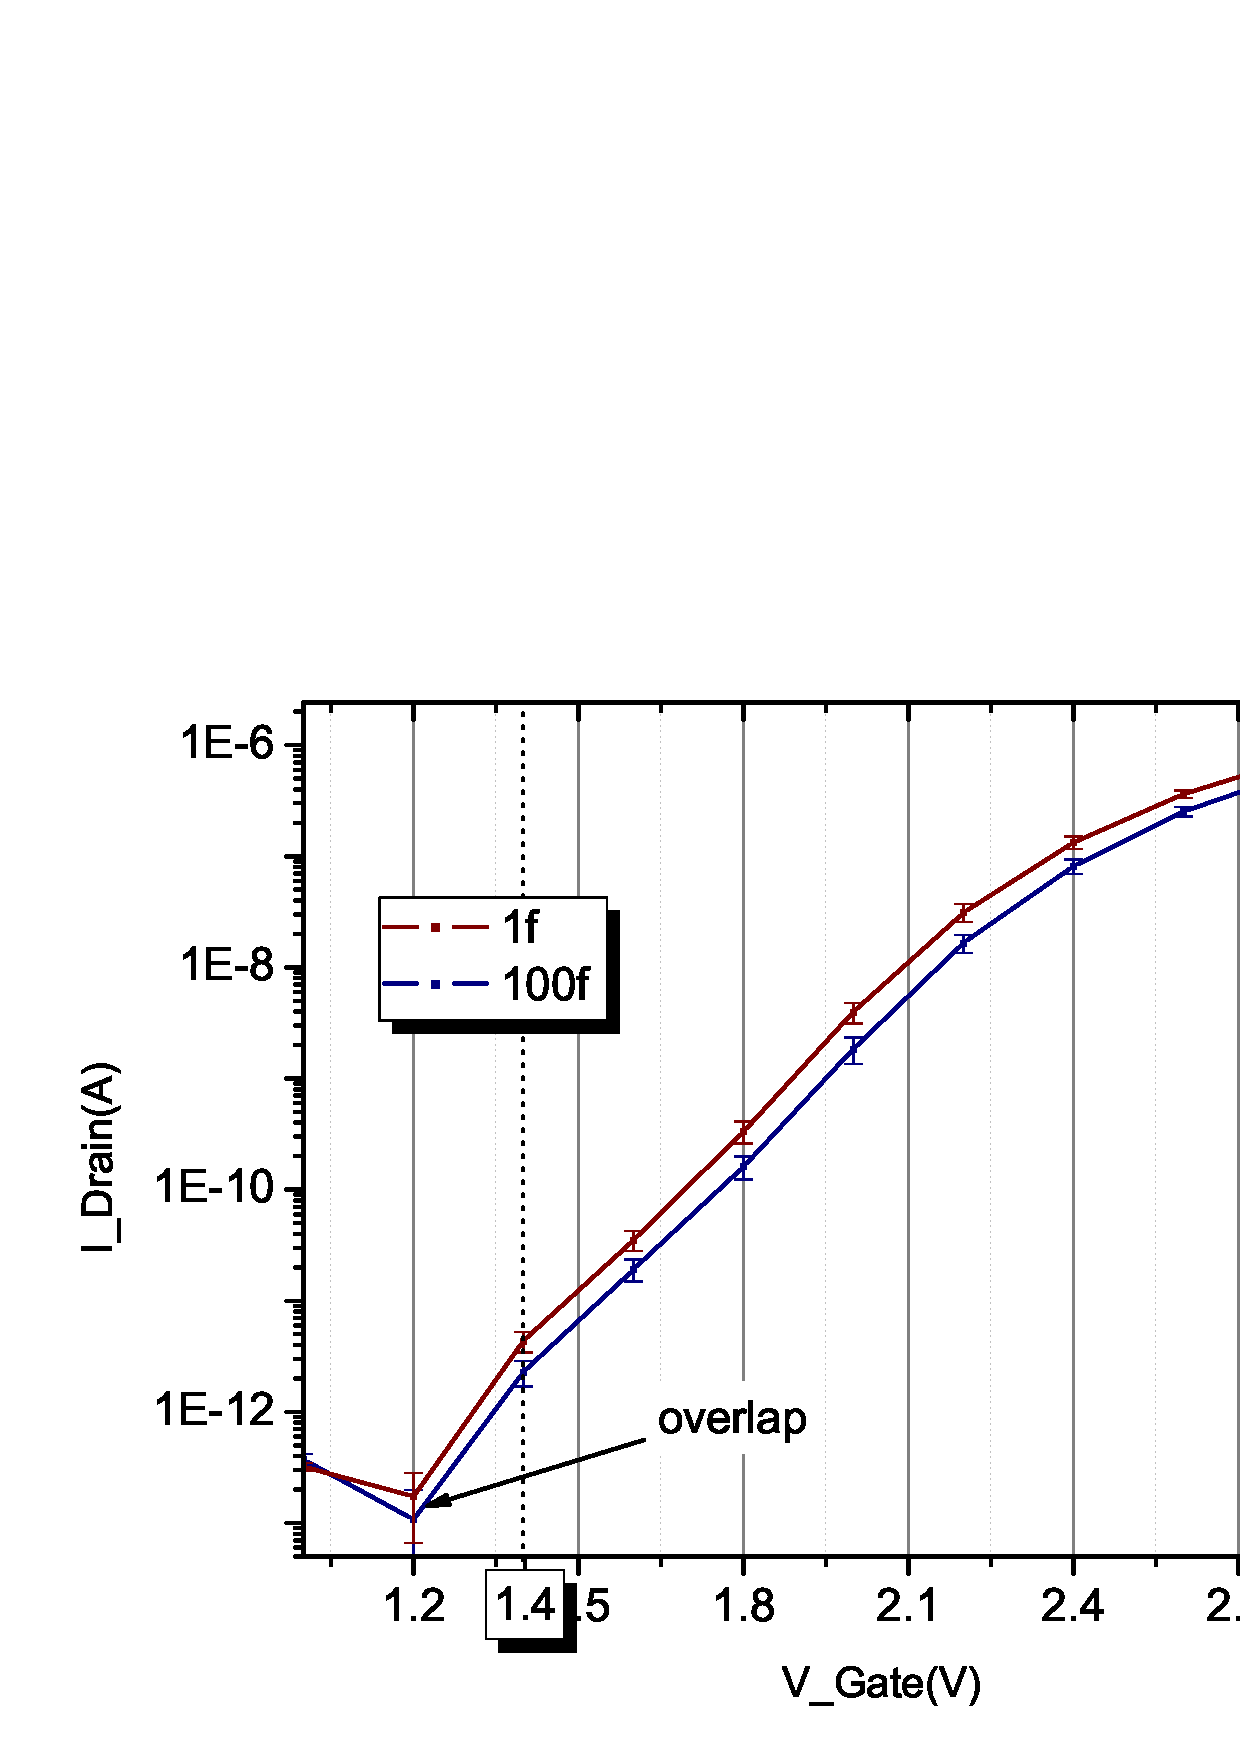
\includegraphics[scale=0.3]{images/chapter3/208_devices/L2-8_log.png}
        (a)
    \end{minipage}
    \hfill
    \begin{minipage}[t]{0.4\textwidth}
        \centering
        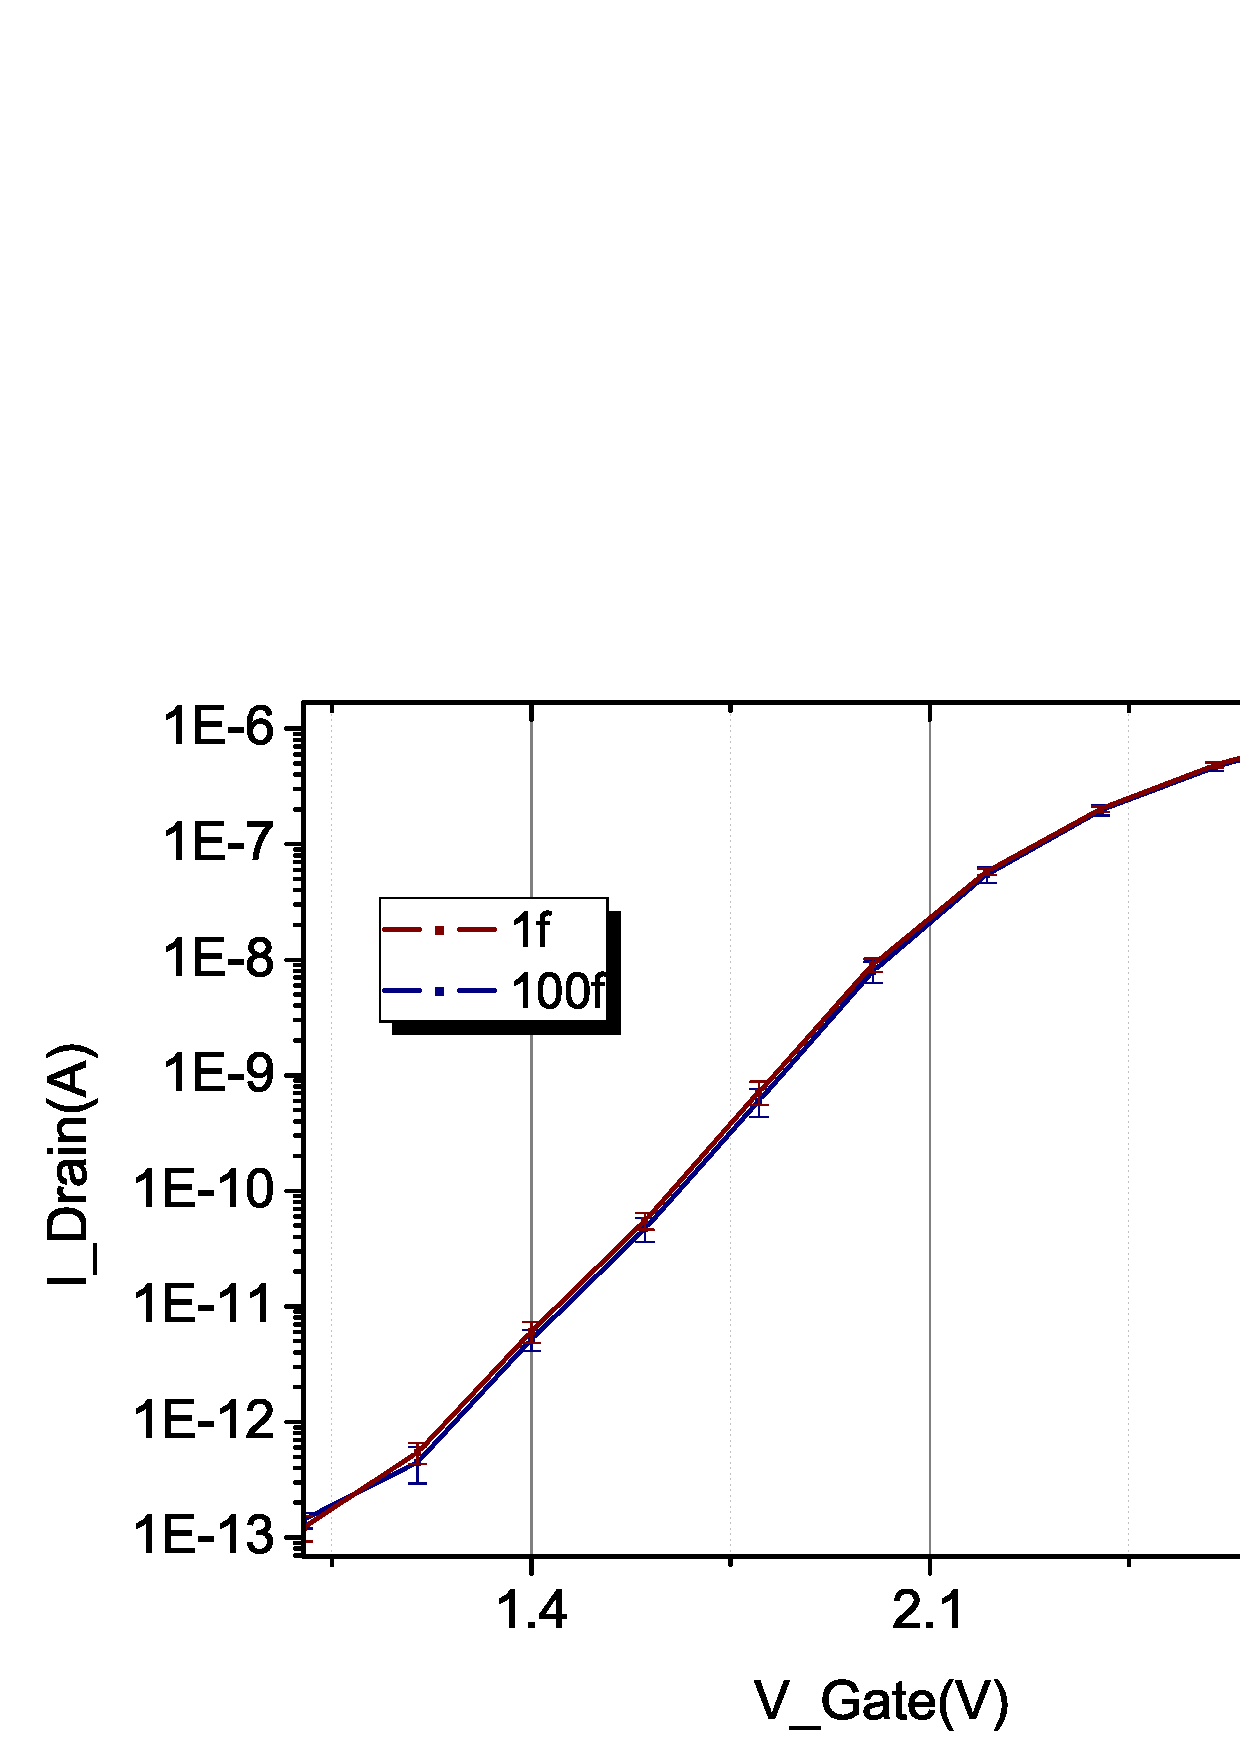
\includegraphics[scale=0.3]{images/chapter3/208_devices/L2-10_log.png}
        (b)
    \end{minipage}
    \caption{Concentration-dependent $I_D$-$V_G$ curves of two equivalent nanowire elements.
    In (a), the measurement result of 1fM and 100fM biomolecule solution is distinguishable. There is no overlap between two curves. This is not true in (b).}
    \label{fig:SD_sucandfail}
\end{figure}

The Fig.\ref{fig:SD_sucandfail} are concentration-dependent measurements (1 femto mole(fM) and 100fM biomolecule solution) obtained with two elements ((a) and (b)).
The two curves in the (a) are distinguishable from the other after gate voltage of 1.4v
They are not distinguishable in the (b) since they overlap each other.
We thus assert that the element of (b) can't detect the concentration difference between 1fM and 100fM.
The noise is stronger than the signal (The signal means the $I_D$ difference caused by the concentration difference).
The element of (a) can do so if it is biased at gate voltage larger than 1.4v or drain current larger than 1E-11.

\begin{figure}[!htbp]
        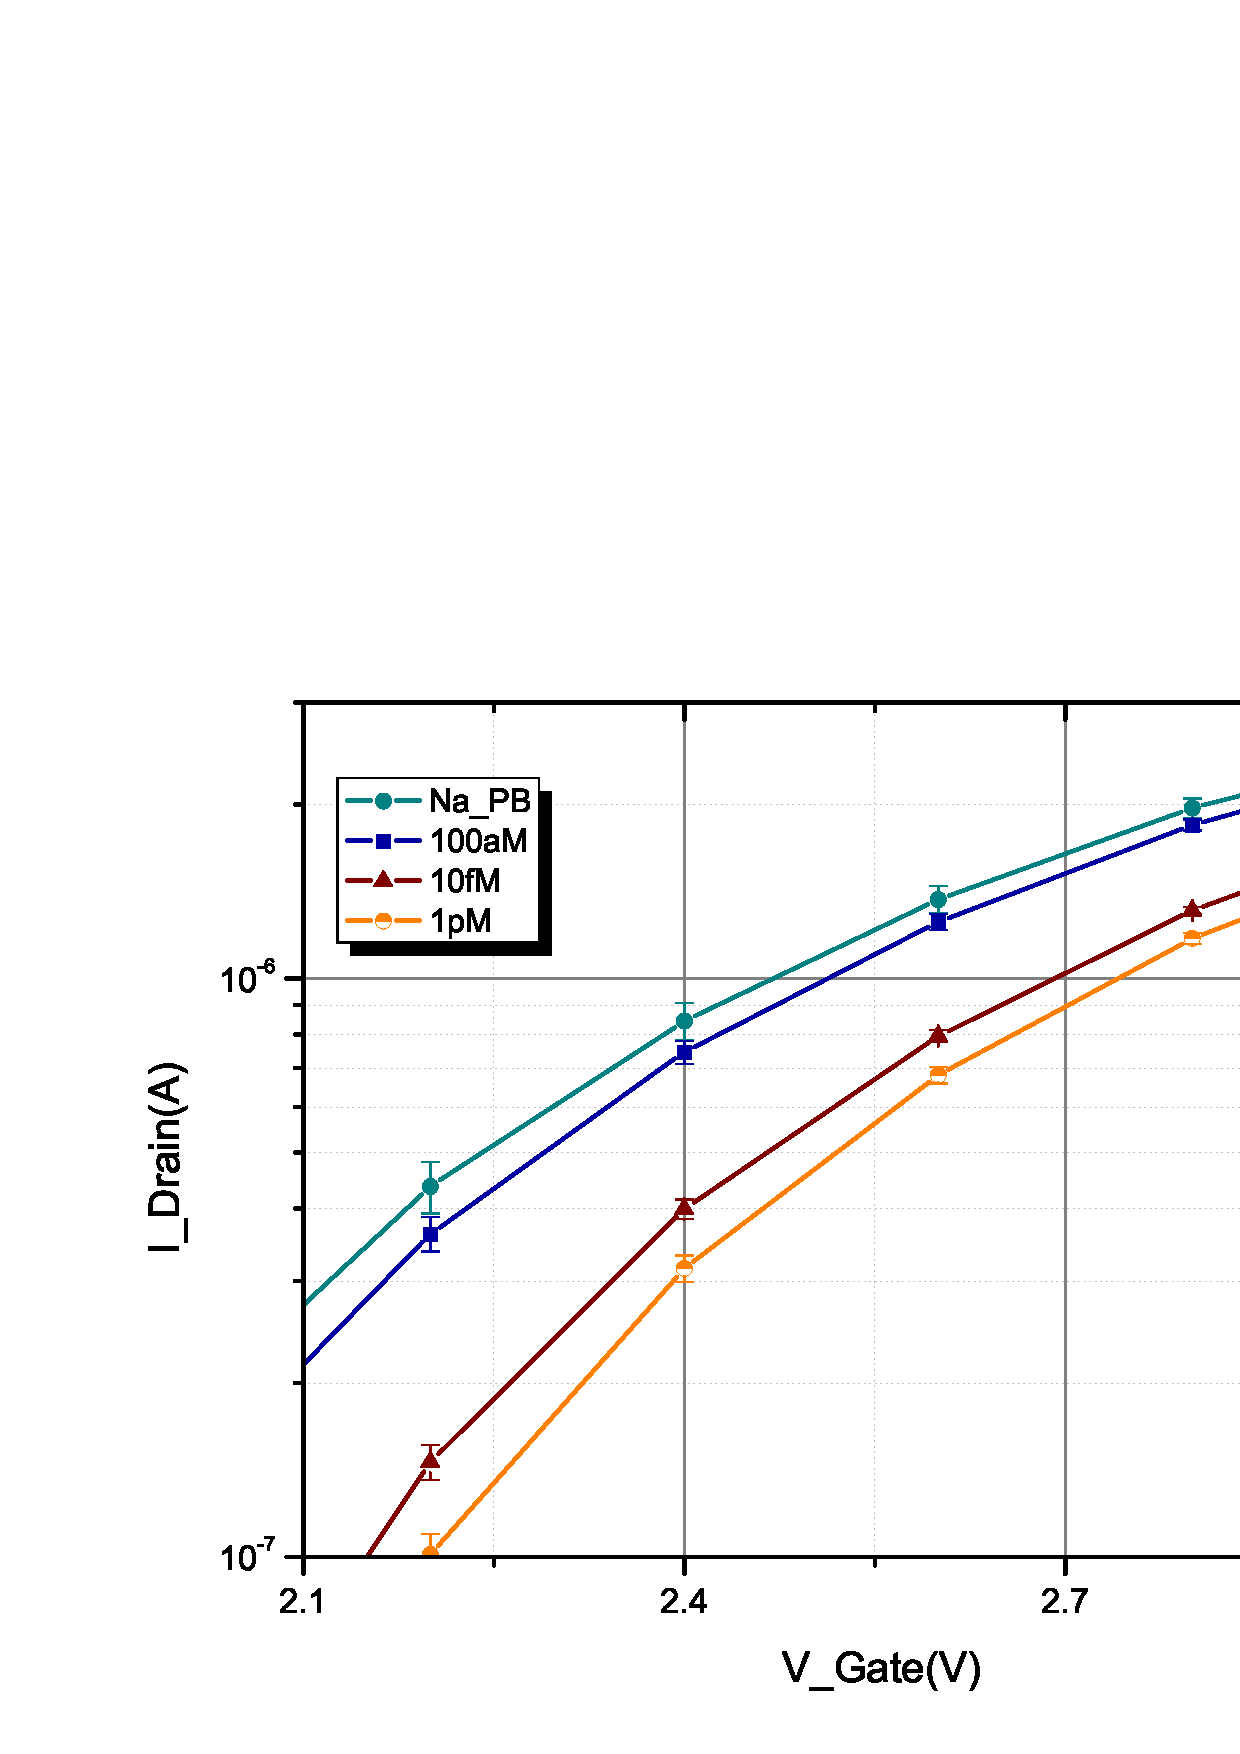
\includegraphics[width=1\textwidth]{images/chapter3/128_allT_mag.png}
    \caption{Concentration-dependent $I_D$-$V_G$ curves.
    Since the biomolecule is negative-charged, the lower the concentration is, the higher the curve is.
    To be noticed, the 10fM curve is closer to the curve of 1pM than 100aM.
     }
    \label{fig:SD_allT}
\end{figure}

In Fig.\ref{fig:SD_allT}, $I_D$ increase with the biomolecule concentration.
One can find that there is only a few ``space'' between PBS buffer and solution containing biomolecule with the concentration of 100aM.
Hence the 100aM should be the limit of detection.

It is worth noting that there is more space between 100aM and 10fM than the space between 10fM and 1pM.
And the noise rate: ${SD} / {Mean}$ is independent of concentration (Fig.\ref{fig:SD_allT2}).
Hence we say that the ``resolution'' for detecting concentration ranging from 100aM to 10fM may be better than the that ranging from 10fM to 1pM.
\begin{figure}[!htbp]
        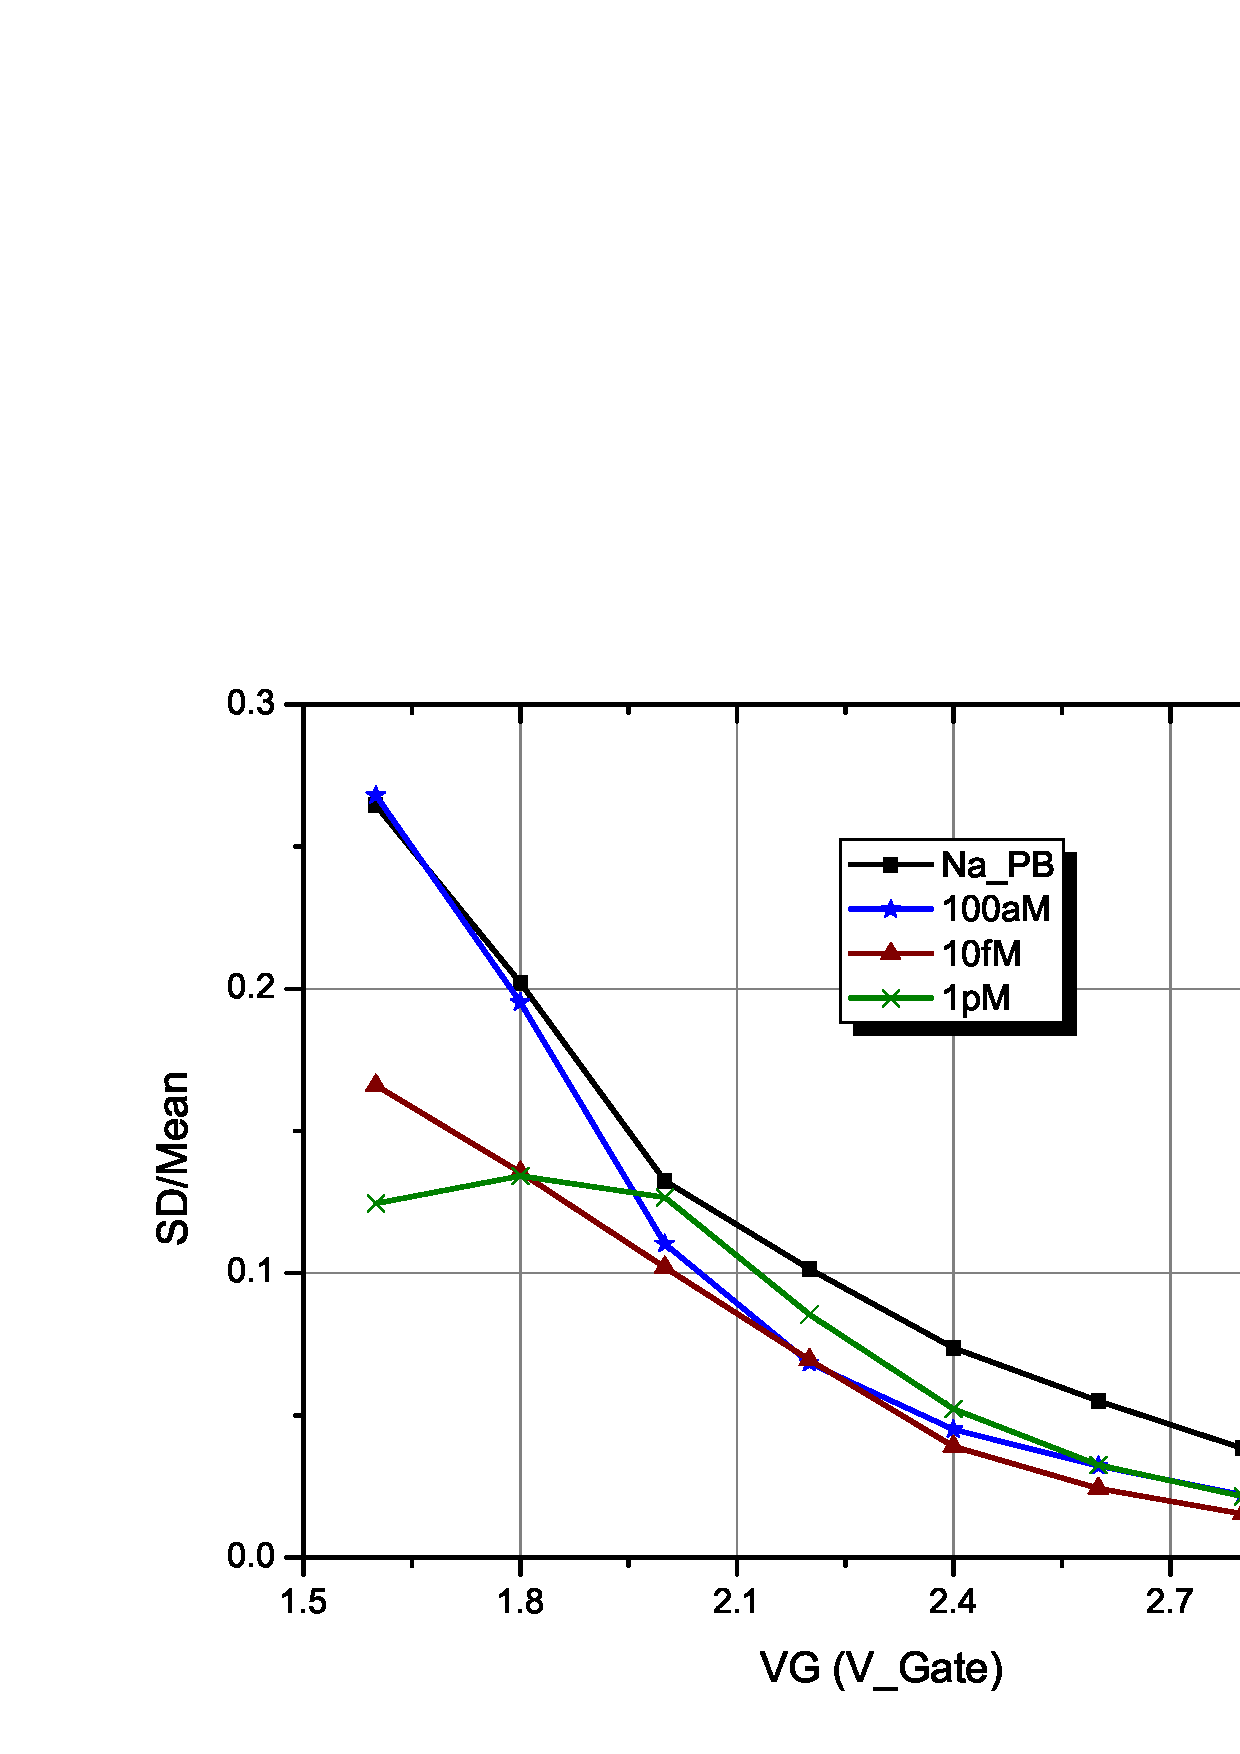
\includegraphics[width=1\textwidth]{images/chapter3/128_allT_error.png}
    \caption{The noise rate of Fig.\ref{fig:SD_allT}. The noise rate is obtained by dividing SD by Mean.}
    \label{fig:SD_allT2}
\end{figure}

\subsection*{Appropriate operation region} \label{section:biasVg}
In \cite{C6}, the team found that ``the induced change of current ($I_D$) following biomolecule was dependent on the applied gate voltage (VG)'' (Fig.).
In other words, a ``biomolecule concentration resolution'' seems to depend on $V_G$
The team tried to find a bias gate voltage range which can induce more current response.
In our opinion, the induced change of current ($I_D$) following biomolecule is not directly dependent on $V_G$.
Based on the our assumption 2 (section\ref{section:twqAssumption}), it depends on the transconductance.
The phenomenon is found by $I_D$-$V_G$ curves, which means the $V_G$ also affect the $I_D$ which cause different transconductance.

Furthermore, we think the noise effect should be taken into consideration.
Some kinds of noise have  positive correlations with transconductance.

Still, we want find an appropriate operation region of nanowire that has the largest concentration resolution.
We proposed a comprehensive method that one should choose the operation region with more ``noise tolerance''.
The noise tolerance is defined as:
\setlength{\mathindent}{2cm}
\begin{align}
    noise \quad tolerance = \frac{I_D1 - SD1 - (I_D2 + SD2)}{I_D2}
\end{align}
$I_D$ and $SD$ are the mean and standard deviation of a curve.
The larger the noise tolerance implies there is more space between two curves.
And more space implies the less chance of overlapping between to concentration curves may happens.

We present analysis results from three nanowire elements.
The Fig.\ref{fig:SD_Device}(a), (c), (e) are the $I_D$-$V_G$ curves of three elements and the Fig.\ref{fig:SD_Device}(b), (d), (f) are the noise tolerance respectively.
One can observe in (b) and (d) that there is first a rising trend then followed by a drop as gate voltage decrease.
The drop doesn't exist in (f) may because the weak inversion is too narrow.
The transistor enters into the reverse region before the drop appears.
The highest points of (b) and (d) locate in the weak inversion region and is close to the transition region (The region between strong inversion and weak inversion region).
We therefore suggest that in this section nanowire should has the largest concentration resolution.


\begin{figure}[!hbtp]
    \centering
    \begin{minipage}[t][20cm][t]{1\textwidth}
        \begin{minipage}[t]{0.3\textwidth}
            \centering
            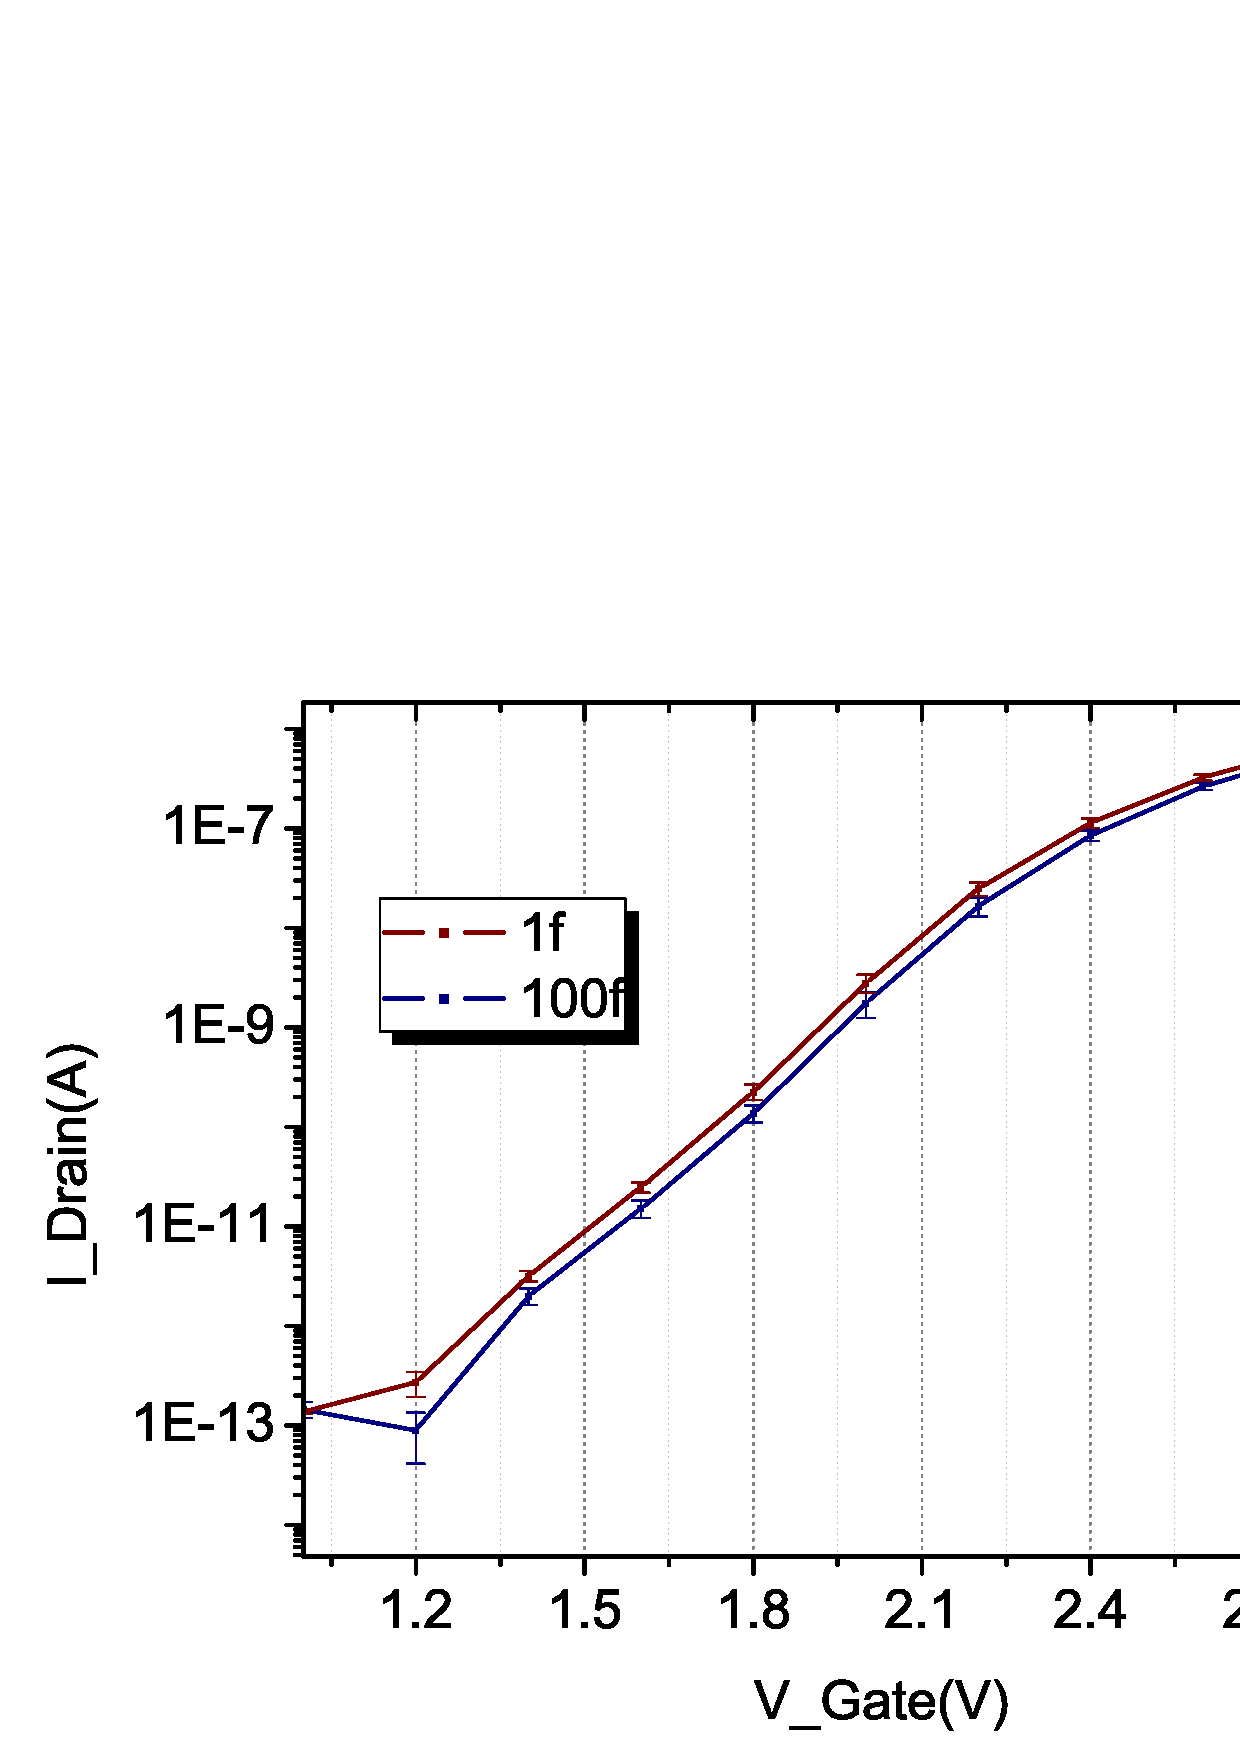
\includegraphics[width=1.8\textwidth]{images/chapter3/208_devices/L2-7_log.png}
            (a)
        \end{minipage}
        \hfill
        \begin{minipage}[t]{0.3\textwidth}
            \centering
            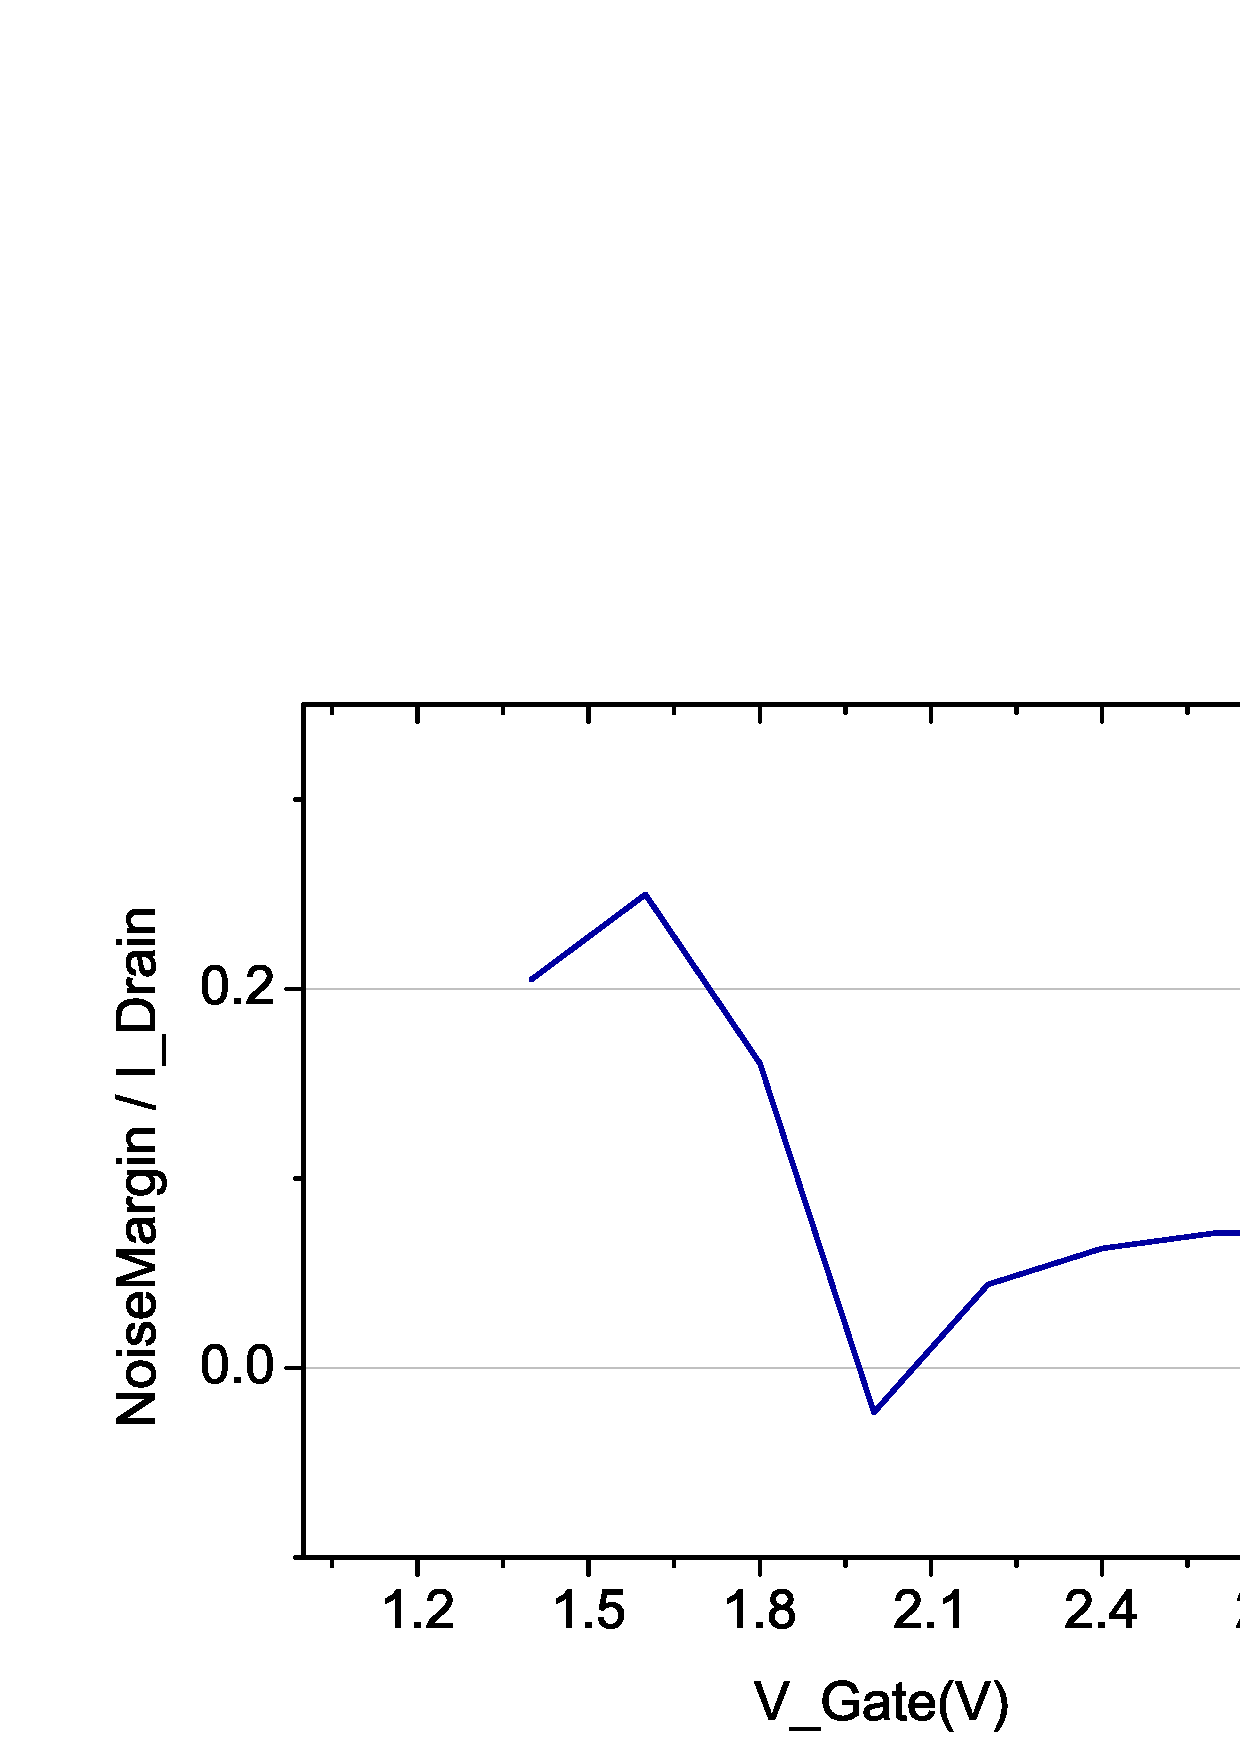
\includegraphics[width=1.6\textwidth]{images/chapter3/208_devices/L2-7_margin.png}
            (b)
        \end{minipage}
        \vfill
        \begin{minipage}[t]{0.3\textwidth}
            \centering
            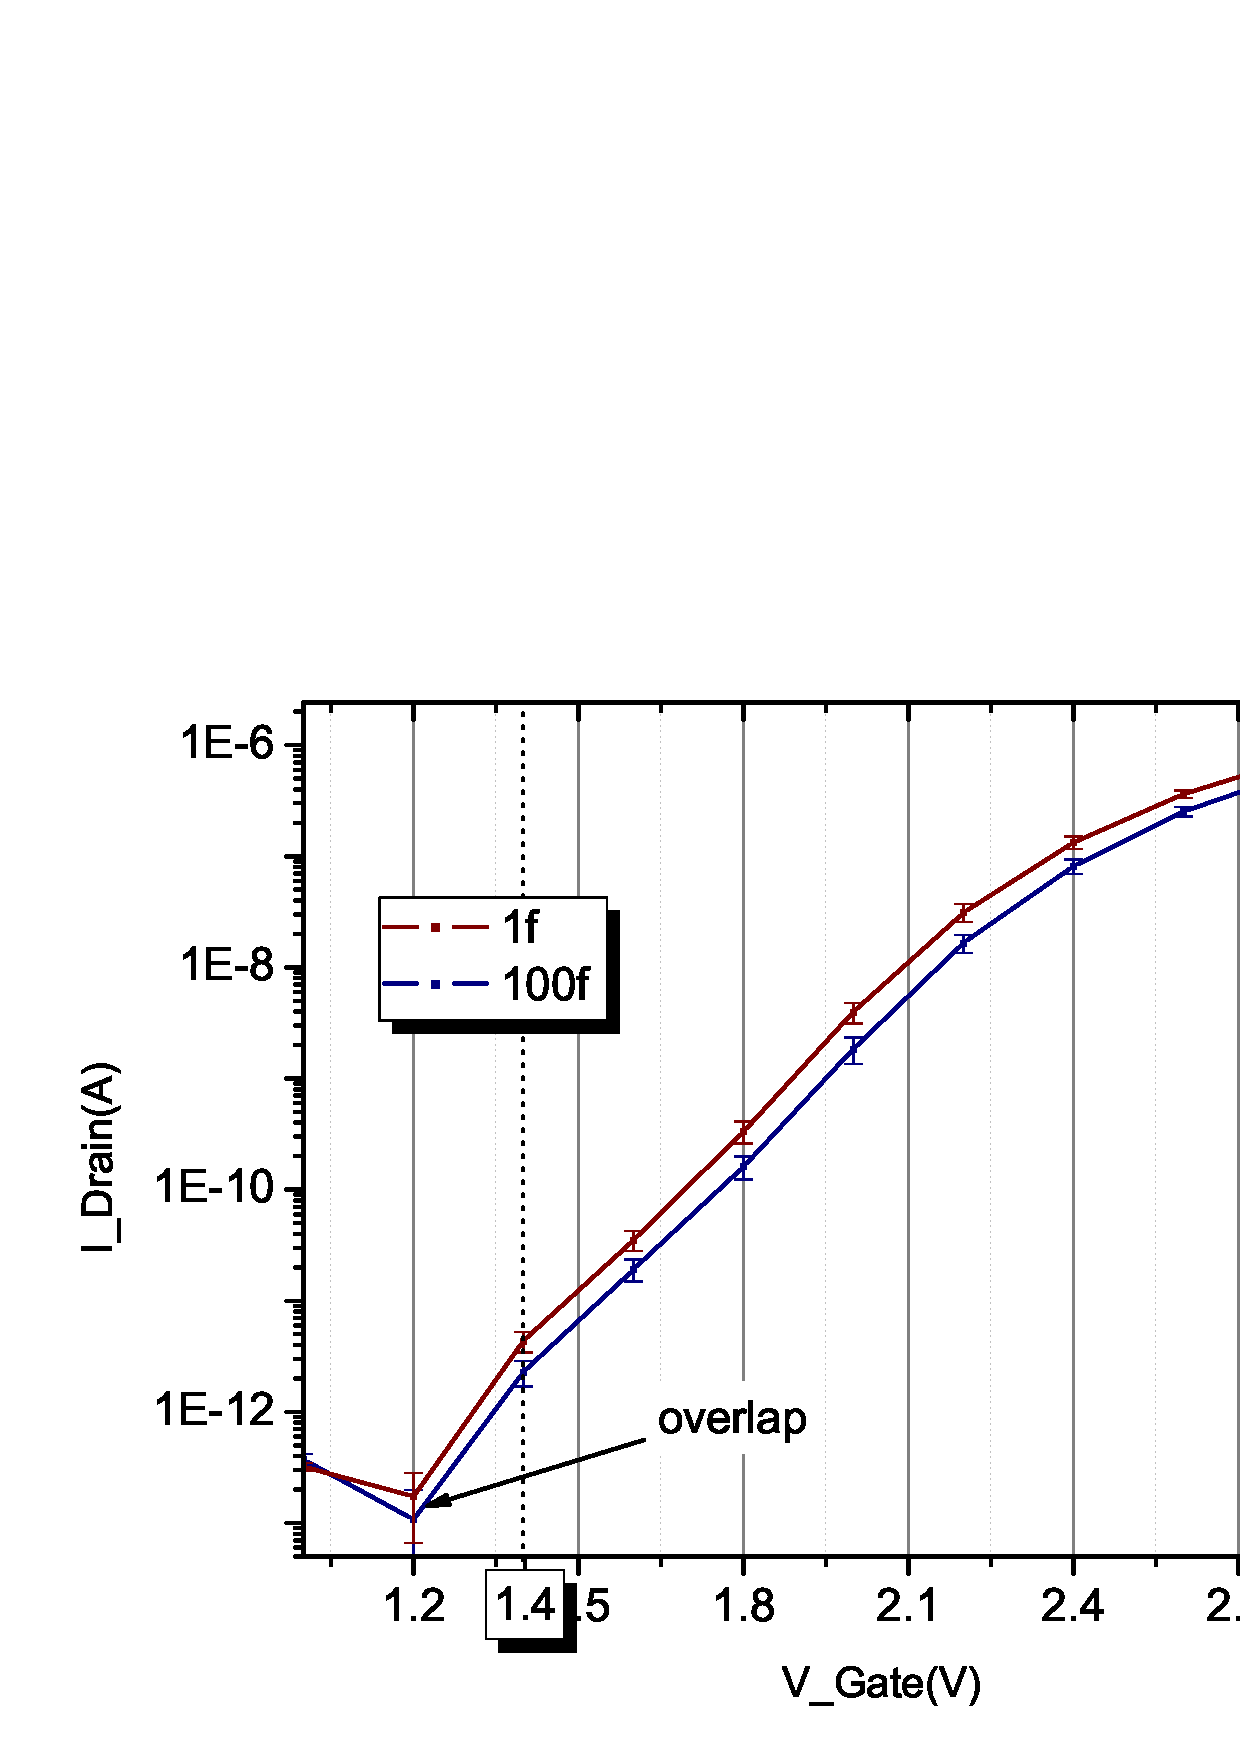
\includegraphics[width=1.8\textwidth]{images/chapter3/208_devices/L2-8_log.png}
            (c)
        \end{minipage}
        \hfill
        \begin{minipage}[t]{0.3\textwidth}
            \centering
            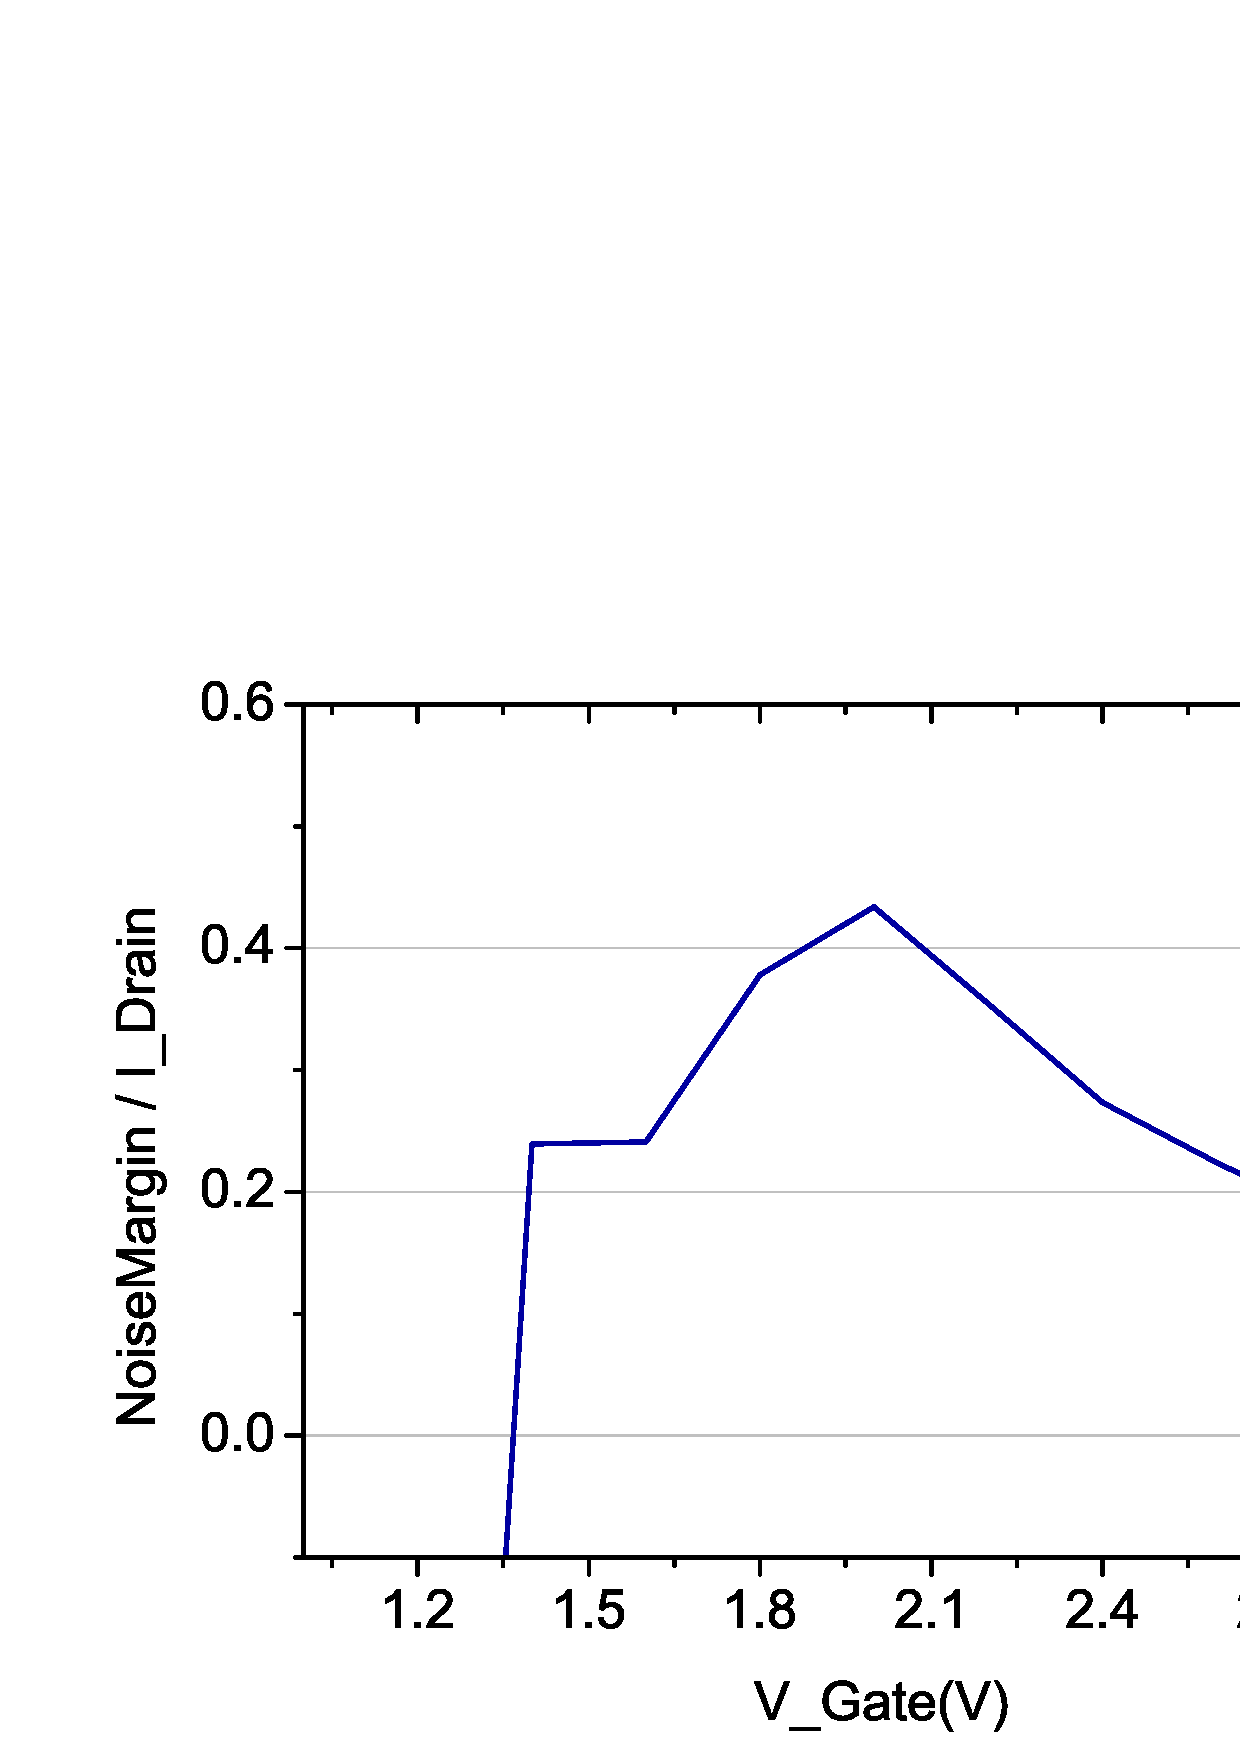
\includegraphics[width=1.6\textwidth]{images/chapter3/208_devices/L2-8_margin.png}
            (d)
        \end{minipage}
        \vfill
        \begin{minipage}[t]{0.3\textwidth}
            \centering
            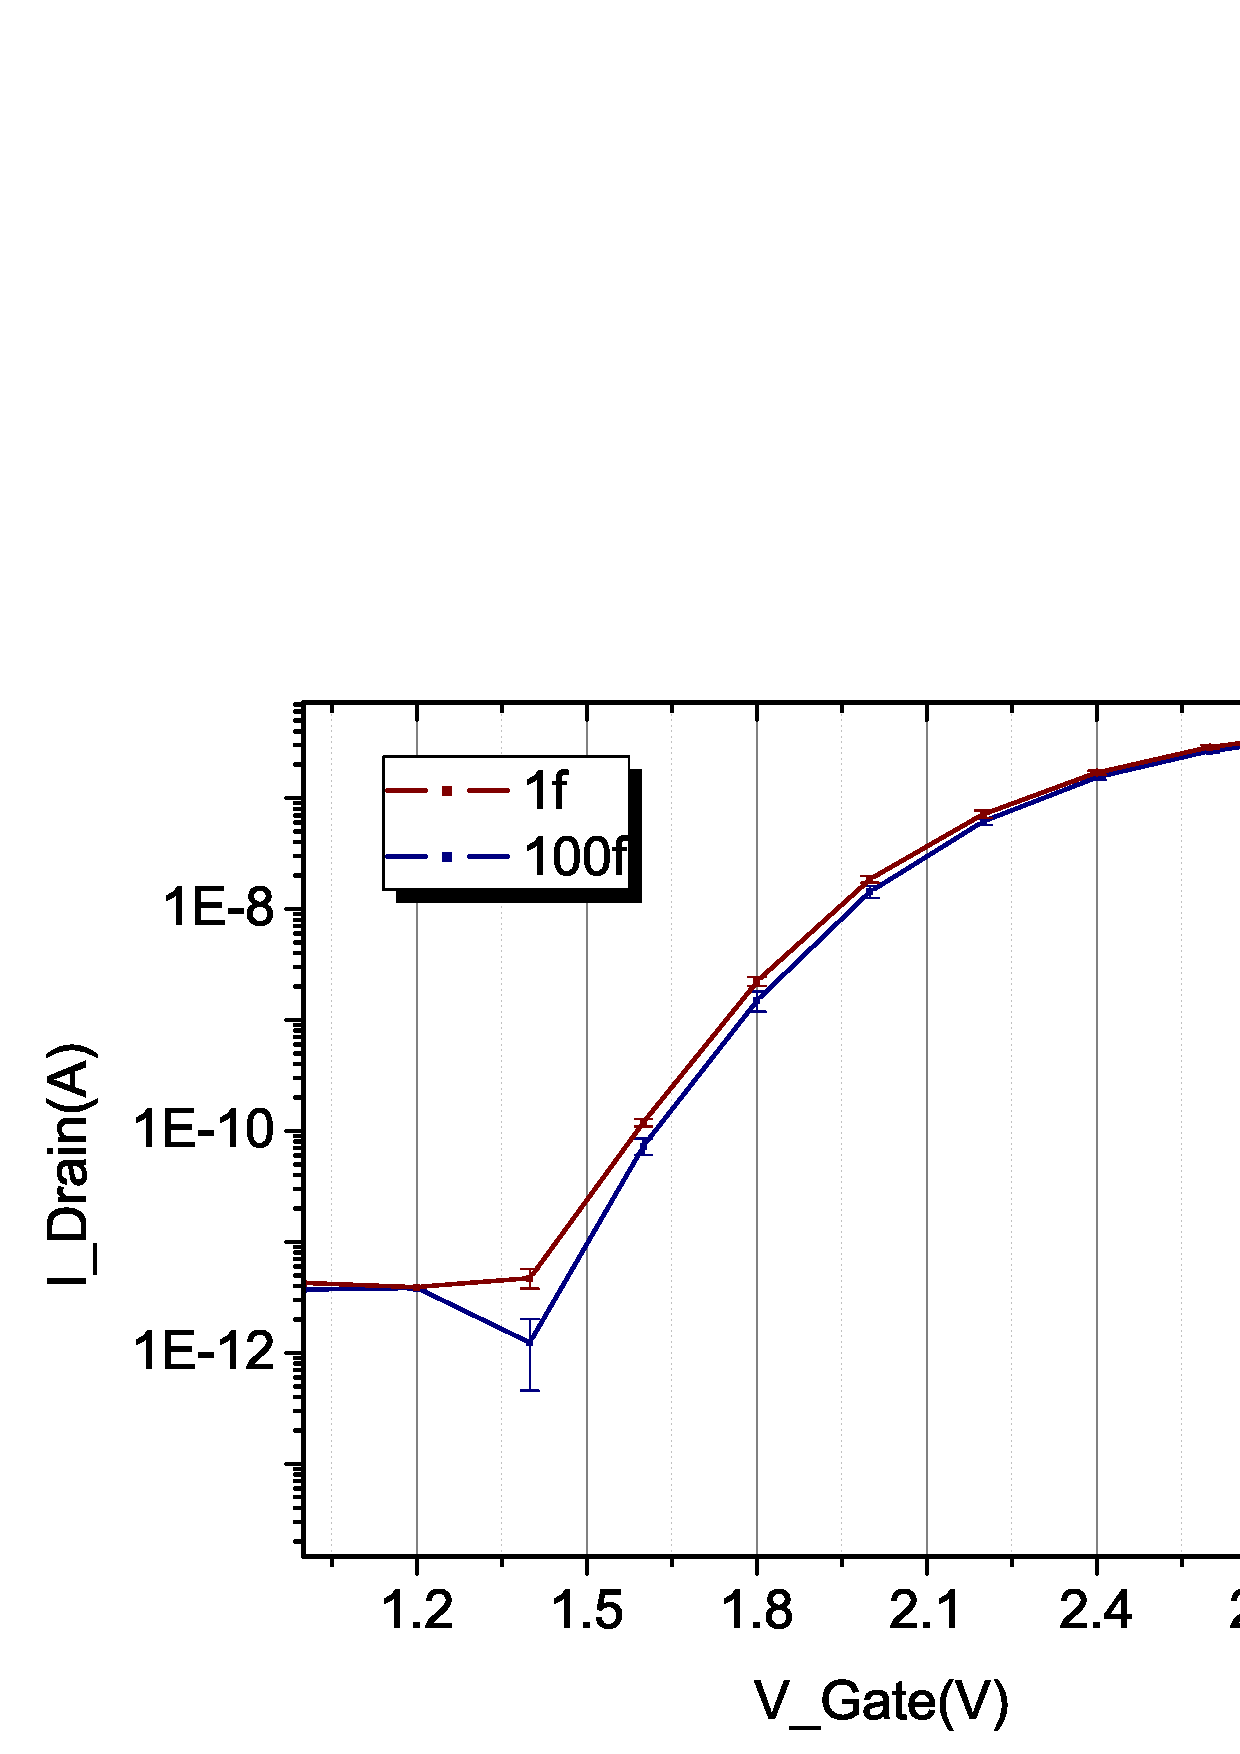
\includegraphics[width=1.8\textwidth]{images/chapter3/208_devices/L2-12_log.png}
            (e)
        \end{minipage}
        \hfill
        \begin{minipage}[t]{0.3\textwidth}
            \centering
            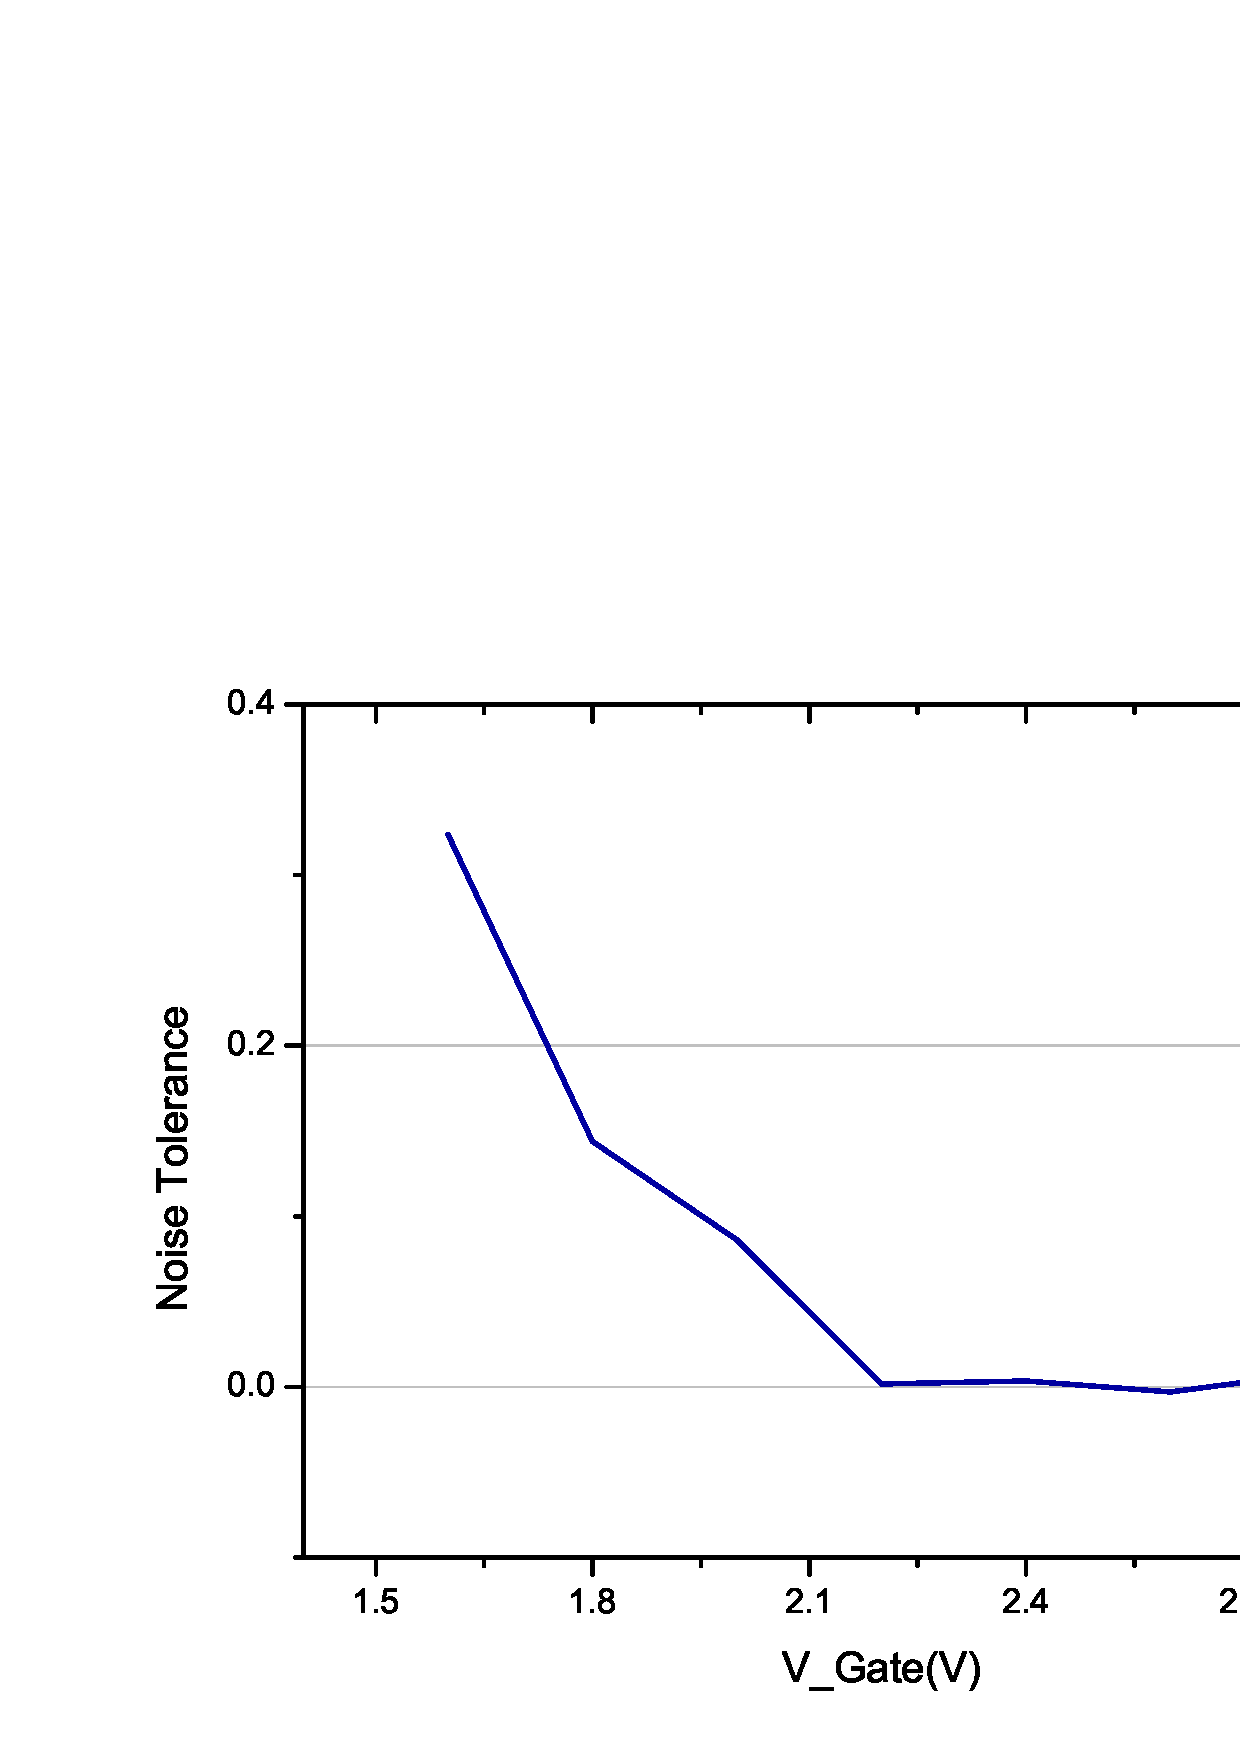
\includegraphics[width=1.6\textwidth]{images/chapter3/208_devices/L2-12_margin.png}
            (f)
        \end{minipage}

    \end{minipage}
    \caption{}
    \label{fig:SD_Device}
\end{figure}



\section{Electrical Measurements}
This section presents the data analysis results.
The data are obtained from our measurements with the source meter (Keithley 2602).
To exclude the ion effect, we placed nanowire elements in dd-water instead of biomolecule solution.
And their poly-silicon channel surfaces are only processed with {\color{red}OH ions.}

\subsection{Front Gate and Back Gate}
Our nanowire has two gates available: floating gate (liquid gate) and back-gate.
We choose floating gate as the operation gate mainly because the floating gate can induce larger drain-current.
In other words, it has higher transconductance (Fig.\ref{fig:IdVgandgbsId}).
In our circuit design, nanowire is placed in a feedback loop where its transconductance is proportional to the loop gain (chapter 5).

\begin{figure}[!htbp]
    \centering
    \begin{minipage}[t][0.1\textheight]{0.4\textheight}
        \centering
        \def\svgwidth{14cm}
        \fontsize{6}{15}\selectfont
        \input {images/FgBg_Compare_Id.pdf_tex}
        (a)
    \end{minipage}
    \hfill
    \begin{minipage}[t][0.1\textheight]{0.4\textheight}
        \centering
        \def\svgwidth{14cm}
        \fontsize{6}{15}\selectfont
        \input {images/FgBg_Compare_Id_dev.pdf_tex}
        (b)
    \end{minipage}
    \caption{Comparison between the DC sweep of voltage on the floating gate and back gate. (a) $I_D$ (b) Transconductance ($g_m$): the derivative of $I_D$}. The traansconductance of the floating gate is larger than the back gate.
    \label{fig:IdVgandgbsId}
\end{figure}


There are some advantages of back-gate.
One of them is the ability to lower the 1/f noise \cite{C7, C8}.
However, this only happens in a very high gate voltage, which is not practical in the integrated circuit design.

\subsection{Transconductance}
The most crucial parameter for our circuit design is the transconductance ($g_m$).
We acquire it by finding the partial derivative of $I_D$ of $V_{G}$.
Since in section.\ref{section:IdGm} we proved that $g_m$ is related to $I_D$, we plot the $g_m$-$I_D$ curve to reveal their relation (Fig.\ref{fig:pIdVg}(b)).

\begin{figure}[!htbp]
    \centering
    \begin{minipage}[t][0.1\textheight]{1\textwidth}
        \centering
        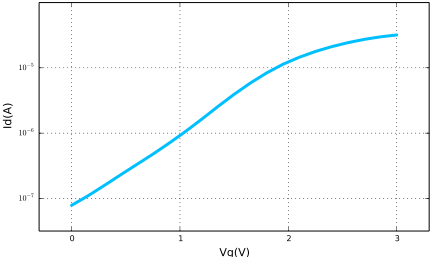
\includegraphics[width=0.6\textwidth,natwidth=610,natheight=442]{images/pIdVg.png}
        (a)
    \end{minipage}
    \hfill
    \begin{minipage}[t][0.1\textheight]{1\textwidth}
        \centering
        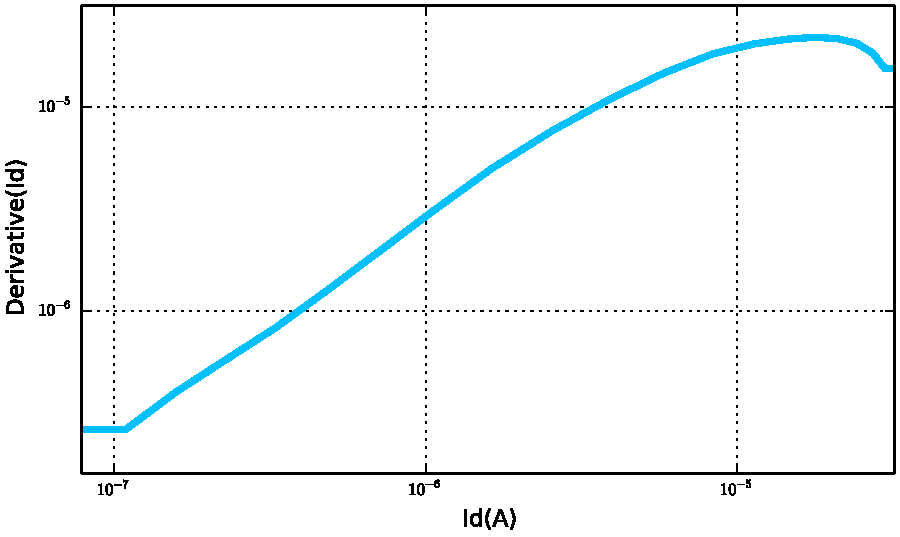
\includegraphics[width=0.6\textwidth,natwidth=610,natheight=442]{images/pIdgbs.png}
        (b)
    \end{minipage}
    \caption{Eelectrical response of a nanowire element. (a) Sweep $V_G$ and measure the $I_D$ changes. And by finding the transconductance ($g_m$): the derivative of $I_D$ of $V_G$, we plot (b) the $g_m$-$I_D$ curve}
    \label{fig:pIdVg}
\end{figure}

The $g_m$-$I_D$ plot indicates that there is a ``linear region'' where $g_m$ is proportional to $I_D$.
This corresponds to our induction (Eq.\ref{eq:gm_weak}).
We can recognize that our nanowire element is operated in weak inversion region when $I_D$ is less than 10$\mu$A.
Therefore, by the section.\ref{section:biasVg}, we decide our the $I_D$ of our nanowire should be operated below 10$\mu$A.

We also proved that the transconductance under this region is unaffected by the $V_{DS}$.

\begin{figure}[!htbp]
    \centering
    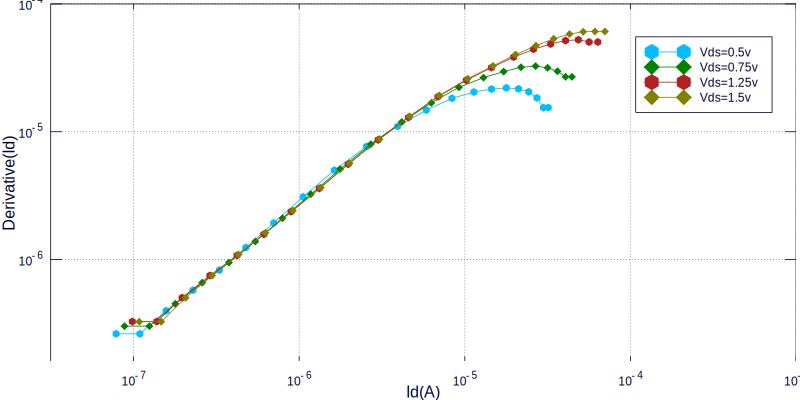
\includegraphics[width=0.8\textwidth]{images/pIdgbs_Vd.png}
    \caption{Id-transconductance with Vds variance}
    \label{fig:Idgbs_Vd}
\end{figure}

\subsection{Drain-to-source impedance ($r_{ds}$)}
In our circuit design, we keep $V_{DS}$ constant.
By the measurement in last section, 0.7 is enough to keep nanowire in saturation region for $V_G$ range from 0v to 3v.
However, due to the fabrication variance, the value varies from 0.75v to 1v.

We concern about how the $I_D$ effect $r_{ds}$.
The way we obtained $r_{ds}$ is as follows:
\begin{enumerate}
    \item Perform $I_D$-$V_G$ sweep with two different $V_D$.
    \item Find the difference of $I_D$ at each $V_G$ sweep point and divide it by the difference of $V_D$.
\end{enumerate}
The result is as Fig.\ref{fig:rds}

\begin{figure}[!htbp]
    \centering
    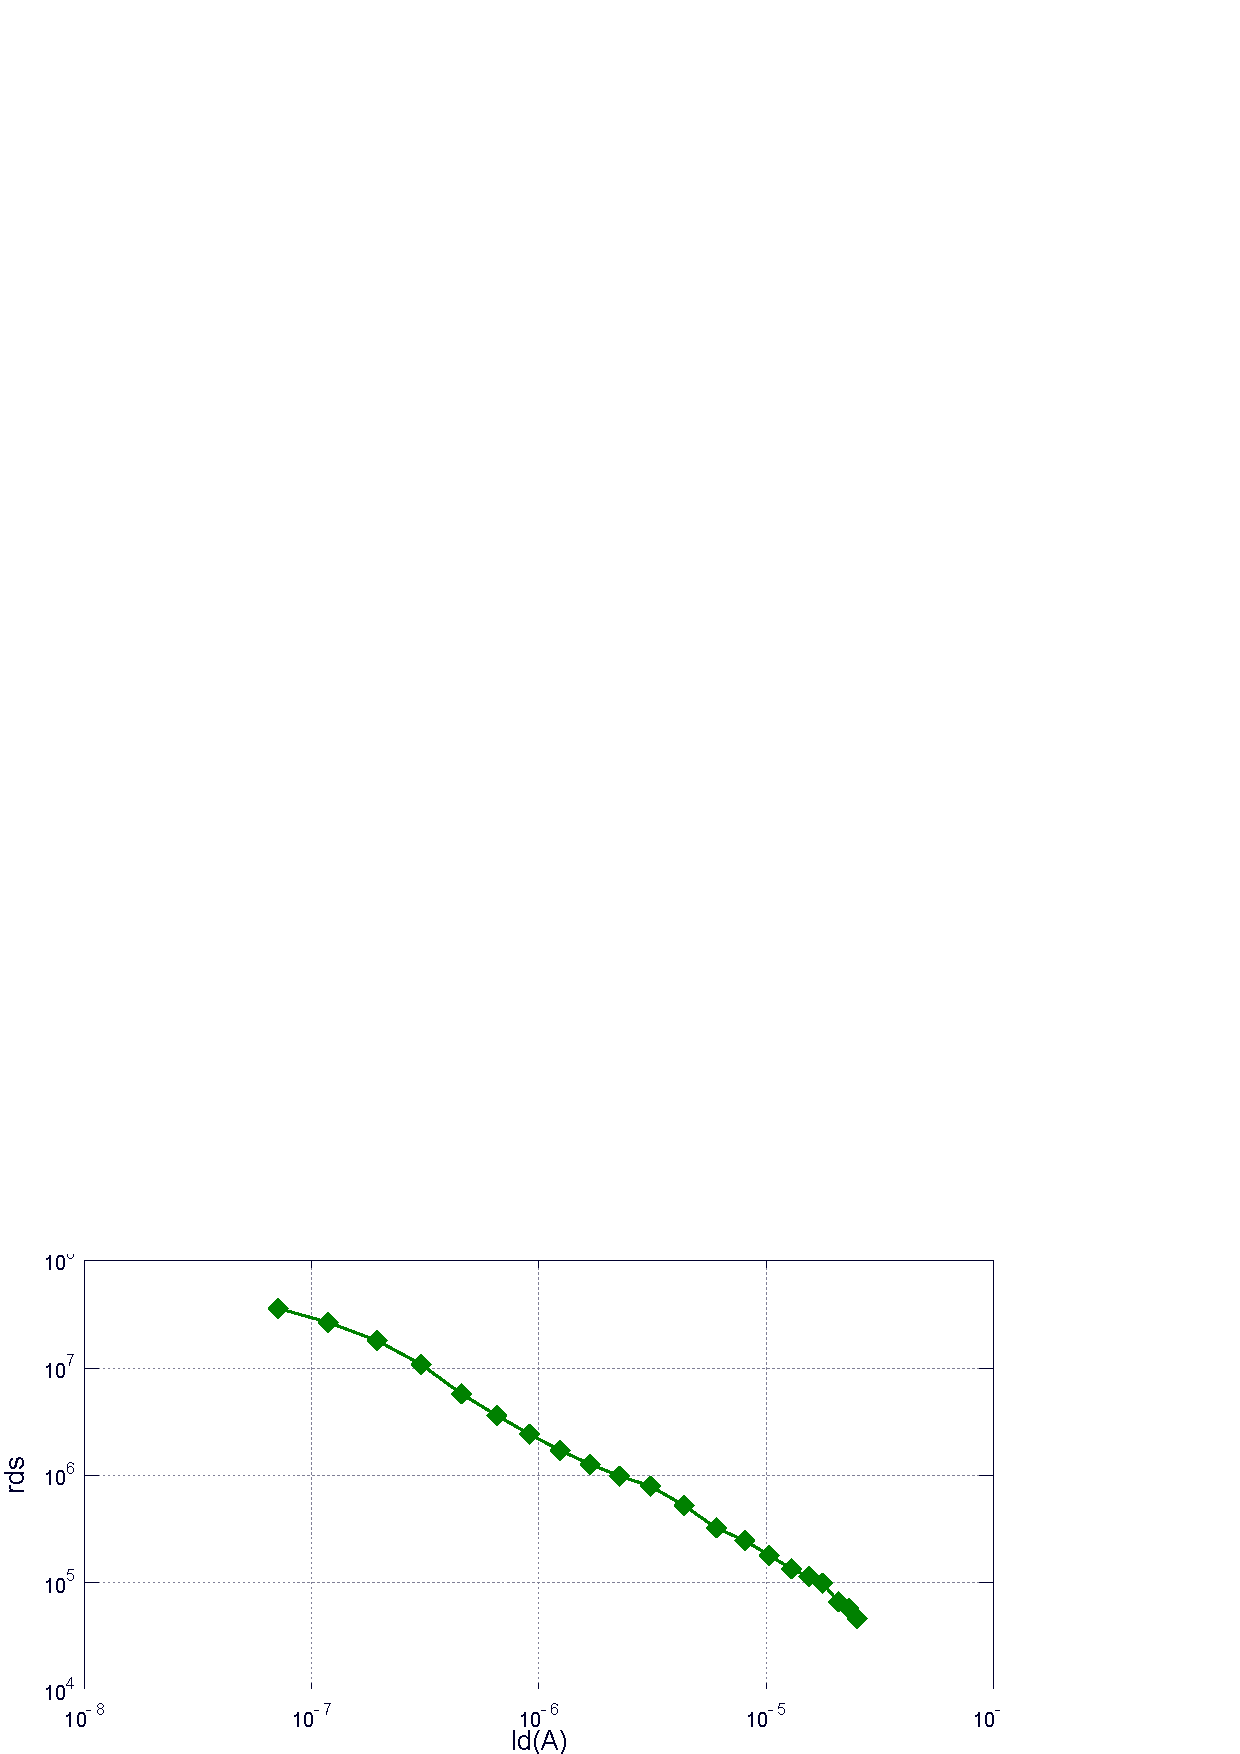
\includegraphics[width=0.8\textwidth]{images/chapter3/rds_I.png}
    \caption{Id-transconductance with Vds variance}
    \label{fig:rds}
\end{figure}


\section{Disparity}
We measured two nanowire elements which lie on the same wafer and are immersed with the same testing PBS solution.
Below the $g_m$-$I_D$ plot (Fig.\ref{fig:disparity}) shows that even the environment is same, two elements exhibit different electrical response.

\begin{figure}[!htbp]
    \centering
    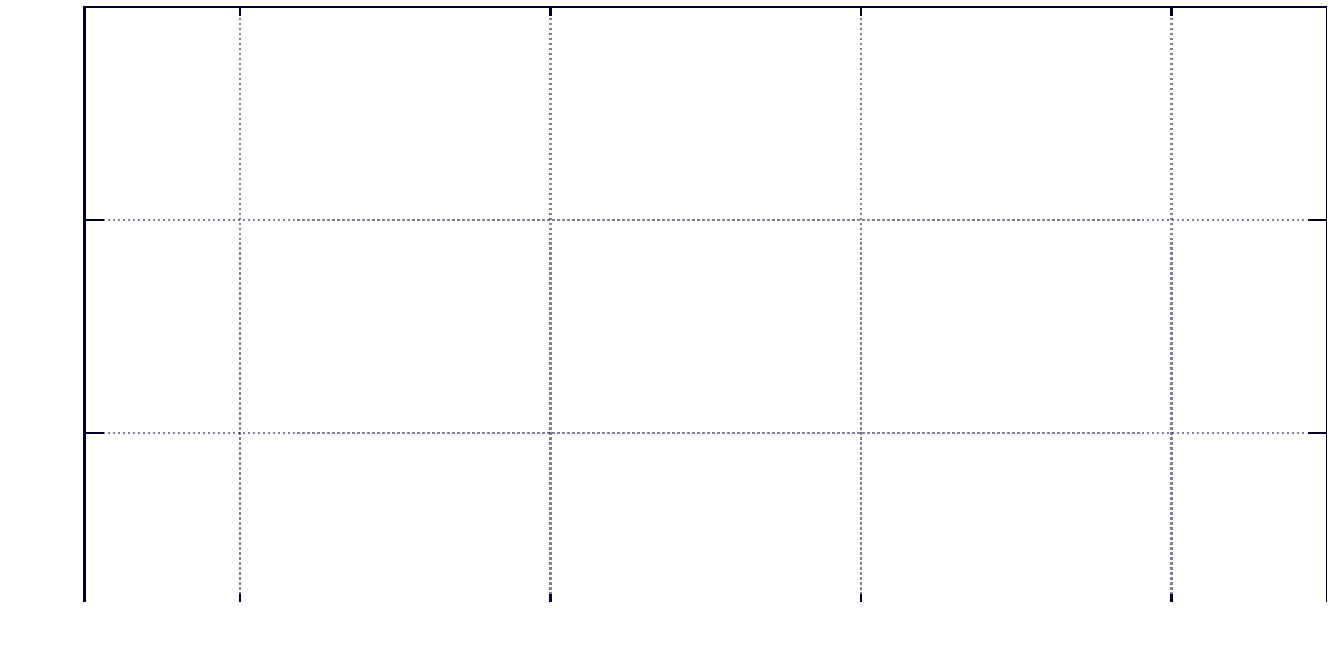
\includegraphics[width=0.8\textwidth] {images/pDisparity.png}
    \caption{Dusparity problem casue nanowire elements with same environment can exhibit different electrical responses.}
    \label{fig:disparity}
\end{figure}










 


\chapter{Discrete Circuitry Design}
This chapter contains the discrete circuit which has been briefly reviewed in section \ref{section:SF}.
We built this circuit to apply the constant-current constant-voltage ($V_{DS}$) method to our nanowire device.

\section{Transforming the design from p-type measuring into n-type measuring}
In \cite{SF1}, the circuit is for p-type ISFET device (Fig.\ref{fig:SF_schematic_old}).
Our nanowire device is n-type.
Hence we transformed the circuit into the one in Fig.\ref{fig:SF_schematic}.
\begin{figure}[!htbp]
    \centering
    \includegraphics[width=0.8\textwidth] {../images/chapter4/SFdiscrete_old.png}
    \caption{The schematic of read-out circuit from \cite{SF1}. The ISFET is a p-type device. It is controlled by the current source $I_b$ whose sub-circuit is shown at right.}
    \label{fig:SF_schematic_old}
\end{figure}
\begin{figure}[!htbp]
    \centering
    \includegraphics[width=0.8\textwidth] {../images/chapter4/SFdiscrete_schematic.png}
    \caption{Our circuit schematic transformed from Fig.\ref{fig:SF_schematic_old}. The device under test (DUT) is a n-type device. It is controlled by the current source $I_b$ whose sub-circuit is shown at right.}
    \label{fig:SF_schematic}
\end{figure}


\section{Circuit Description}
The circuit is divided into two sections: the constant-voltage circuit and the constant-current source (Ib).

\subsection*{The constant-voltage circuit}
The constant-voltage circuit section has a source follower structure.
The input of the circuit is at the floating gate ($G$) of the device under test (DUT), where the output is at its source ($S$).

The $I_D$ of DUT is controlled by Ib.
Because The leakage current flowing into the negative input of OP2 is less than 0.1nA, the $I_D$ of the transistor should always be same as the current provided by Ib.

The $V_{DS}$ of DUT is always equal to the potential difference ($I_0 \times R_0$) across the resistor $R_0$.
This is achieved by two OP-based, unity-gain buffer.
They connected serially with $R_b$ and cause the voltage at the drain ($D$) to follow the voltage at the source ($S$).


\subsection*{The  constant-current source (Ib)}
The Ib circuit is in fact a current scaling down circuit.
By concerning the OP as ideal, the node $OP+$ has the same voltage as $OP-$.
This equalizes the potential difference between two resistors whose resistance are different by $N$-fold.
As a result, the currents $I_b$ and $I_s$ are also different by $N$-fold.
$I_b = I_s / N$.

The capacitor is for filtering. It filters the high frequency noise out to create a stable output current.


\section{Discrete Element}
We use tlc2264 made by Texas Instrument (TI) as our OP.
This OP requires a supply voltage of $\pm 5v$ and can perform rail-to-rail output operation.
Its open-loop gain (Large-signal differential voltage amplification rate) is 170 for the output load greater than 50k.

\begin{figure}[tb!hp]
    \centering
    \includegraphics[width=0.3\textwidth]{images/chapter4/LM334.png}
    \caption{LM334: The discrete element we use for current source Is. It has three terminals: $R$, $V_+$, $V_-$. The output current ($I_s$) flows from $V_+$ to $V_-$. The resistor $R_{SET}$ connected to $V_-$ and $R$ is for adjusting the output current.}
    \label{fig:lm334}
\end{figure}

\emph{For the current source Is and I0, we use lm334 (Fig.\ref{fig:lm334}) made by National Semiconductor.
It is a 3-terminal adjustable current sources with a wide dynamic cross voltage range of 1v to 40v (the cross voltage $V_{+} - V_{-}$ in Fig.\ref{fig:lm334}), and current accuracy of $\pm 3\%$.
In our experiment, the current $I_s$ is fixed at $1\mu A$ with an output impedance of $1.2G\Omega$.}


\section{Circuit Performance and Conclusion}
We examined the performance of our circuit by plotting its $I_D$-$V_G$ curve.
The $I_0$, $R_0$ and $V_G$ were kept constant.
We swept $I_D$ by changing the $N$ value with a variable resistor.
$N$ ranges from 1 to 1000.
And $I_b$ should range from $1\mu A$ to $1n A$.

We measured the output voltage at $S$ and subtracted this value from $V_G$ to get the corresponding $V_{GS}$.
These two values gave the $I_D$-$V_{GS}$ curve in Fig.\ref{fig:SF_result}.
We compare this curve with the curve obtained by directly sweeping $V_G$ and measuring $I_D$ with Source Meter (Keithley 2602).

\begin{figure}[!htbp]
   \centering
   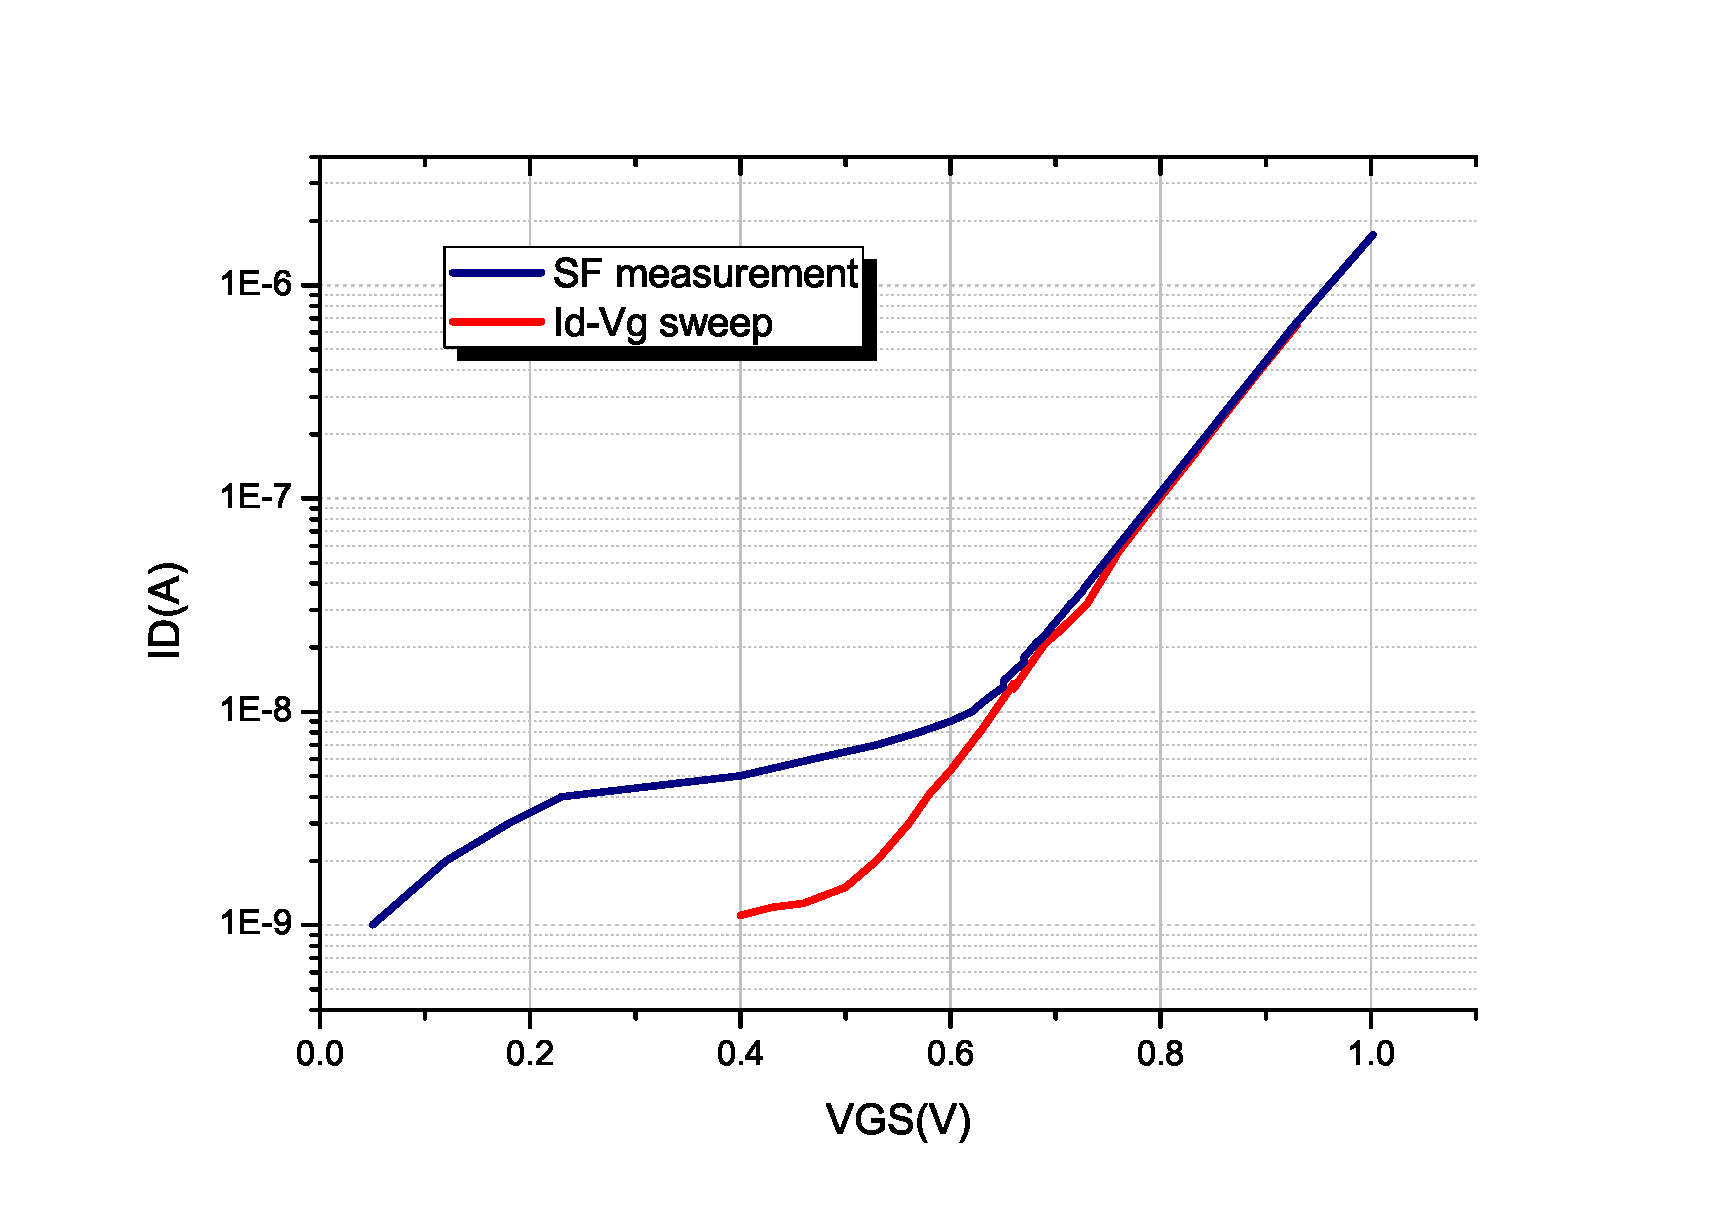
\includegraphics[width=1\textwidth]{images/chapter4/SF.eps}
   \caption{The measuremet result (``SF\_measurement'') compares with the direct $I_D$-$V_G$ sweep (``Id-Vg sweep'').}
   \label{fig:SF_result}
\end{figure}

The result shows that when $I_D$ is larger than $10n A$, the circuit is functional.
Two curves are same as each other.

The circuit fails when $I_D$ is smaller than $10n A$.
This is related to the impedance matching between the constant-voltage circuit and the Ib circuit, which we have discussed in section.\ref{section:SF}.

The output impedance of the Ib circuit is:
\begin{equation} \label{eq:rcs2_again}
    N\times R_s
\end{equation}
$R_s$ is the output impedance of the current source Is which equals to $1.2G\Omega$.
And the current input impedance at the $S$ of the constant-voltage circuit is:
\begin{equation} \label{eq:rsf2_again}
    \frac{1}{g_m}
\end{equation}

We plot the $I_b$-Impedance relationship in Fig.\ref{fig:SF_imp}.

\begin{figure}[!htbp]
   \centering
   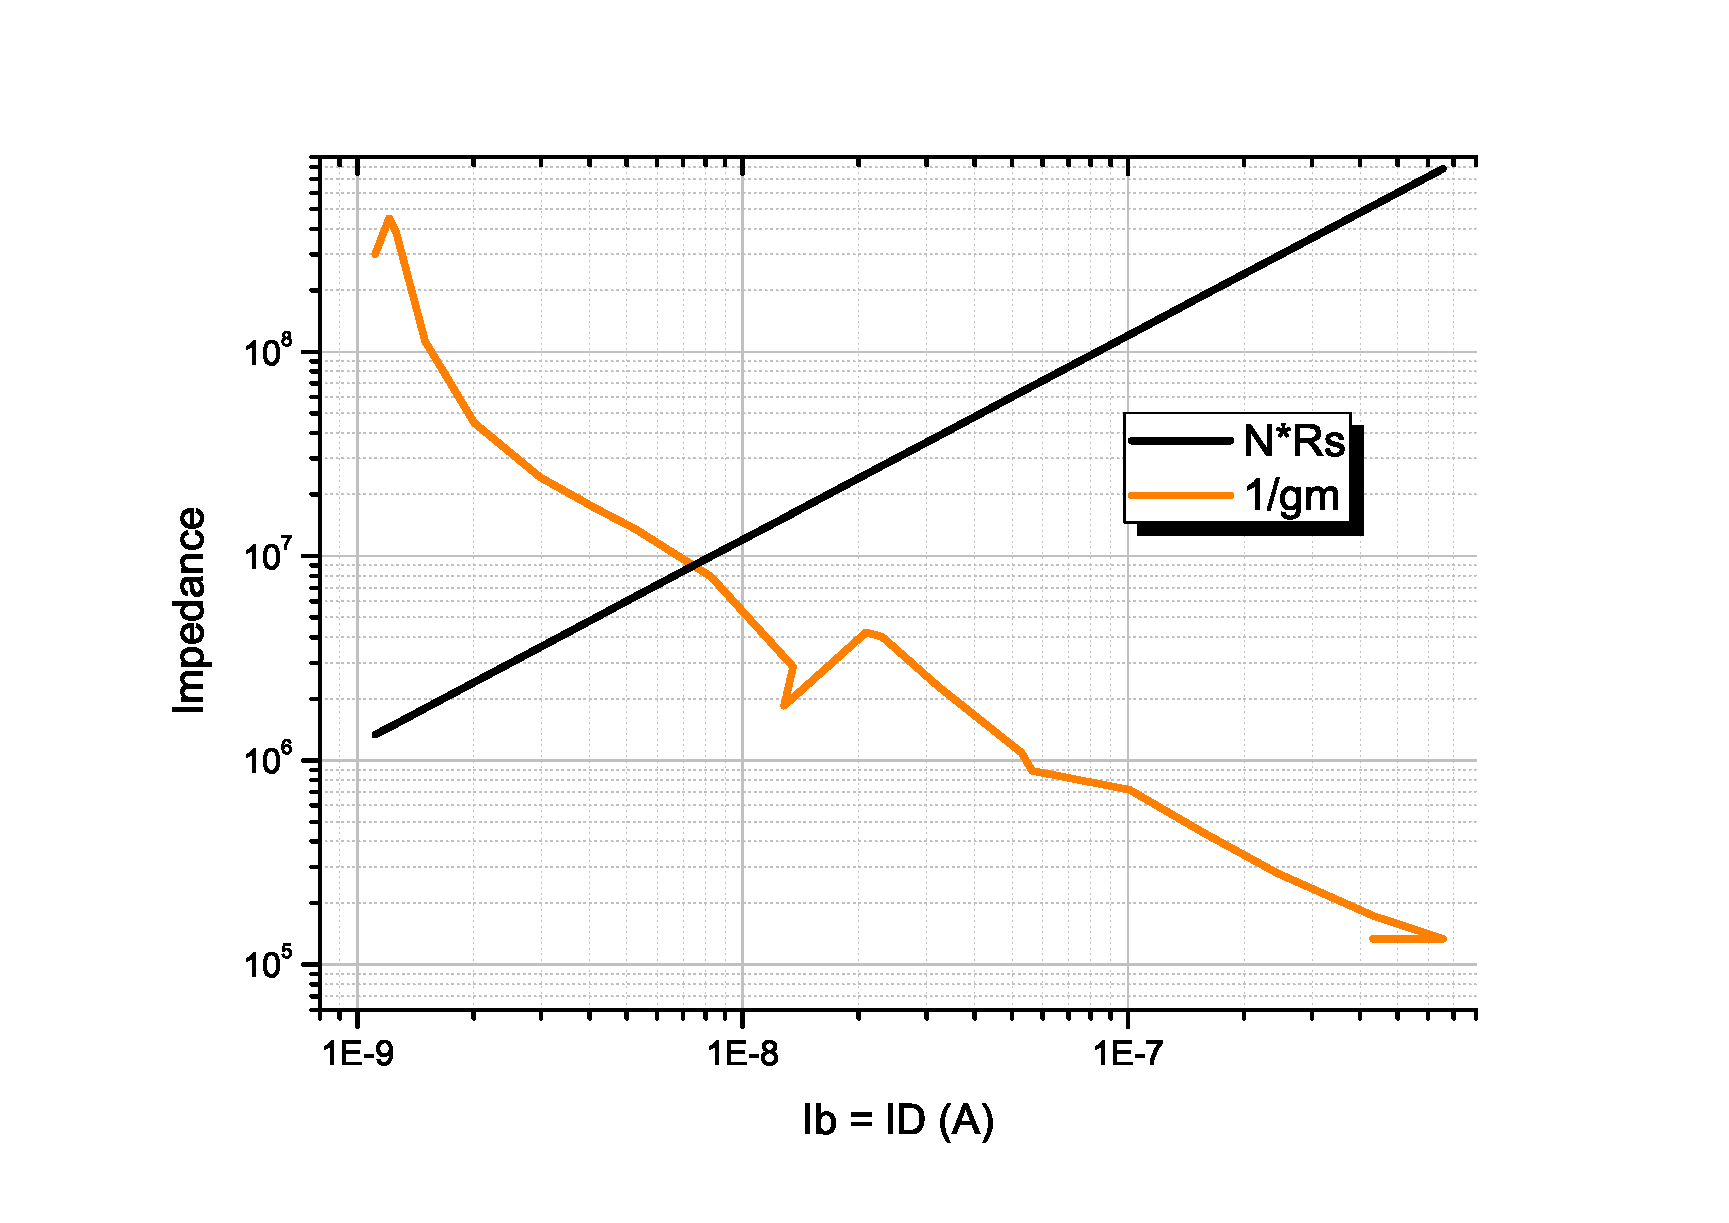
\includegraphics[width=1\textwidth]{../images/chapter4/SF_impedance.eps}
   \caption{Input impedance of transistor (``1/gm'') and output impedance of Ib circuit (``N * Rs''). The former is found by the derivative of $I_D$ of $V_{Gs}$. The latter is obtained by Eq.\ref{eq:rcs2_again}.}
   \label{fig:SF_imp}
\end{figure}


It shows that the output impedance of Ib is close to the input impedance of transistor when current is $10n A$ (N = 100).
The impedance is unmatched.

Overall, the constant-current constant-voltage method is feasible.
What one needs to notice when applying the this method is the impedance matching.
In the source follower structure, its current input impedance varies with the bias current.
It affects the dynamic range and needs more design concern.



\chapter{Integrated Circuitry Design}
This chapter presents the design of the read-out circuit and the simulation results.


\section{Architecture}
The review of source follower in section.\ref{section:SF} suggests the constant current method for the circuit of DC measurement.
The data analysis from chapter 3 supports it by the linear relation between $I_D$ and $g_m$.
However, the section.\ref{sec:AC} shows that source follower is not suitable for AC measurement.
It alternatively recommends the circuit in Fig.\ref{fig:lockin} which measures ac current signal and converts it into voltage output.
This circuit is appealing because of its noise suppression, simplicity and flexibility.

We combined these two method into one circuit structure and introduce them below.

\subsection{Circuit Schematic: First Stage}

\begin{figure}[!htbp]
    \centering
    \includegraphics[width=0.4\textwidth] {images/chapter5/DCMode.png}
    \caption{}
    \label{fig:DCmode}
\end{figure}

\paragraph*{DC mode}
Fig.\ref{fig:DCmode} is the first stage of our read-out circuit connected in DC mode.
As in the source follower, there is a bias current source (Ibias) for controlling the $I_D$.
The difference is that the Ibias inputs the current into drain instead of source.
In addition to this, we apply the TIA from section.\ref{sec:AC} (\cite{Jlockin}).
Its output connects to a rail-to-rail OP amplifier, which forms a negative feedback loop.
When the $I_D$ is greater than the current of Ibias, it lowers the output voltage of TIA and raise the gate voltage $V_G$.
And vice versa.
This is to say that the feedback mechanism forces the $I_D$ be equal to the current of Ibias by adjusting the $V_G$.

\begin{figure}[!htbp]
    \centering
    \begin{minipage}[t]{0.4\textwidth}
        \includegraphics[width=1\textwidth] {images/chapter5/ACMode.png}
        \raggedleft
        (a)
    \end{minipage}
    \hfill
    \begin{minipage}[t]{0.4\textwidth}
        \includegraphics[width=1\textwidth] {images/chapter5/ACMode_sine.png}
        \raggedleft
        (b)
    \end{minipage}
    \caption{}
    \label{fig:ACmode}
\end{figure}

\paragraph*{AC mode}
In Fig.\ref{fig:ACmode}(a), the switch in Fig.\ref{fig:DCmode} turns to a simple voltage source (Vg) which bias nanowire with the gate voltage.
The OP is nonfunctional with its output connected floating.
When performing measurement, we directly find how the solution concentration changes the output voltage ($V_{out}$).
This output voltage will input into the second stage circuit which is for the amplification.

\paragraph*{Dealing with the Disparity Problem}
As mentioned in chapter 1, we combine DC mode and AC mode to perform a disparity-resisting measurement.
Assuming there are two nanowire elements having disparity problem.
Initially, they are applied with DC mode to perform the $I_D$-$V_G$ sweeping.
We calculate their $g_m$ by the derivative of $I_D$ of $V_G$ and find the $g_m$-$I_D$ relation of these elements.
Then we select a $g_m$ value.
For the two elements, this value corresponds to two $I_D$.
And these two $I_D$ corresponds to two $V_G$.
We set the Ibias and Vg to these values.
Finally, after these initialization steps, we add the measuring solutions and detect the difference of $V_{out}$.
Since elements have same $g_m$, they should produce same voltage differences.
Before the next measuring solutions is added, we return to DC mode to find new $V_G$.
This reset $I_D$ of the elements to the value of Ibias, which also reset the $g_m$ to the value we selected.

\paragraph*{Another Usage of AC mode}
There is another way to perform measurement with AC mode, which resembles the method in \cite{Jlockin}.
This method measures the $g_m$ of nanowire.
As in Fig.\ref{fig:ACmode}(b), the source of nanowire is applied with an ac signal ($v_s$).
An ac output in $V_{out}$ is equal to $v_sg_m \times R_{TIA}$.
The values of Ibias and Vg can be arbitrary.
But one need to be aware that the values should not saturate the output of TIA or the second stage circuit.

Below, we talk about some design concept.

\subsubsection{Detecting Range Improvement (AC mode)} \label{sec:Ibias}
In section.\ref{sec:ch2CC} about the TIA subcricuit as Fig.\ref{fig:TIA_old}(a), we mentioned that the detecting range of $R_{NW}$ is limited.
There are same limits in our circuit which detects the current variance of nanowire.
We now discuss the causes of these limits and show the strategies we use.
To be noticed that the TIA block is a two-stage differential input and single output op-amp in the flowing discussion.

\begin{figure}[!htbp]
    \centering
    \begin{minipage}[t]{0.4\textwidth}
        \includegraphics[width=1.1\textwidth] {images/chapter5/TIA_olda.png}
        (a)
    \end{minipage}
    \hfill
    \begin{minipage}[t]{0.4\textwidth}
        \includegraphics[width=1\textwidth] {images/chapter5/TIA_old.png}
        (b)
    \end{minipage}
    \caption{\textbf{(a)} The transimpedance block (TIA) of the readout circuit from \cite{Jlockin}. The circuit input a voltage signal into resistive nanowire element $R_{NW}$.
            To compare it with our circuit (Fig.\ref{fig:TIA}), we transform the voltage input into an equivalent current input in \textbf{(b)}. The $I_{NW} = (V_{Ref} - V_{in})/R_{NW}$ and $\Delta i = \Delta vi /R_{NW}$}
    \label{fig:TIA_old}
\end{figure}

\paragraph*{Lower Limit:}
According to Fig.\ref{fig:TIA_old}(b), the TIA output voltage is:
\begin{equation}
    V_{TIA} = V_{Ref} + I_{NW}R_{TIA} + \Delta iR_{TIA}
    \label{eq:TIA_old}
\end{equation}
Two reasons which result in the lower limit of the detecting range relate to a large offset current $I_{NW}$.
One is that the output current provided by the TIA is restricted by design.
The other is that the restriction of the current flowing through the resistor $R_{TIA}$:
\begin{align}
    \frac{V_{Ref}}{R_{TIA}} < I_{NW} < \frac{VDD - V_{Ref}}{R_{TIA}}
\end{align}
Both reasons leads to the output saturation of TIA.

A naive way to handle the first reason is to increase the output current which TIA can provide.
The side effects of this method are the increases in power consumption and chip area.
As for the second reason, using smaller $R_{TIA}$ can ease the restriction on $I_{NW}$ and reduce the lower limit.
Unfortunately, it reduces the upper limit as well.
This will be discussed in the paragraph of ``upper limit''.

Our strategy for decreasing the lower limit is by utilizing the bias current source of nanowire.
According to Fig.\ref{fig:TIA}, the Eq.\ref{eq:TIA_old} is transformed into:
\begin{equation}
    V_{TIA} = V_{Ref} + (I_{NW} - I_{bias}) R_{TIA} + \Delta iR_{TIA}
    \label{eq:TIA}
\end{equation}
Now we can diminish the large $I_{NW}$ by Ibias.
In conclusion, the large offset current cause the saturation of the output of TIA.
We use the biasing current source to diminish that offset current, which increase the detecting range.

\begin{figure}[!htbp]
    \centering
        \includegraphics[width=0.4\textwidth] {images/chapter5/TIA.png}
    \caption{}
    \label{fig:TIA}
\end{figure}
\paragraph*{Upper Limit:}
The upper limit issues from the output resolution.
If the signal $\Delta iR_{TIA}$ from Eq.\ref{fig:TIA} is too small, it may be defeated by the noise.
One may be raise up the SNR by using large $R_{TIA}$.
However, the chip area constrain the size of resistors.
In our circuit design, we cannot make the resistance value out of $100k\Omega$.
Furthermore, even if the resistor can be greater, one need to concern for the noise brought by the large resistance.

Our strategy is to boost the SNR of TIA by designing its input MOSFETs in a large area.
And we also amplify the output signal through the second stage circuit.

\subsubsection{Input impedance Matching (DC mode)}
From the chapter 4, we learned that for the constant current method, the impedance matching between current source Ibias and nanowire element is important.
The matching decides the limit of the biasing current.
Here we calculate the input impedance of the circuit.

\begin{figure}[!htbp]
    \centering
        \includegraphics[width=0.4\textwidth] {images/chapter5/input_imp.png}
    \caption{}
    \label{fig:input_imp}
\end{figure}
In Fig.\ref{fig:input_imp}, by applying and input voltage $\Delta v_x$, we find the $\Delta i_x$.
The input impedance of the circuit is $\Delta v_x / \Delta i_x$.
\begin{align}
      \Delta i_x &= \quad i_D + i_{TIA} \\
      i_D &= \quad \frac{\Delta v_x}{r_{ds}} + \Delta v_xA_{TIA}A_{OP}g_m\\
      i_{TIA} &= \quad \frac {\Delta v_x}{R_{TIA} / (1 + A_{TIA})} \\
      \Delta v_x / \Delta i_x  &= \quad (\frac{1}{r_{ds}} + \frac{1 + A_{TIA})}{R_{TIA}})^{-1} \label{eq:input_imp}
\end{align}
The $A_{TIA}$ is the gain of the opAmp in TIA block.
The $A_{OP}$ is the gain of OP.
The $r_ds$ is the drain-to-source resistance of nanowire which is large than $100k\Omega$.
From the Eq.\ref{eq:input_imp}, we conclude that the input impedance of the circuit is equal to:
\begin{equation}
        \frac{1/g_m}{A_{TIA}\times A_{OP}}|| r_{ds} || \frac{R_{TIA}}{1 + A_{TIA})}
\end{equation}

In out design, the Ibias is an simple pmos.
Its output impedance roughly ranges from $1M\Omega$ to $1G\Omega$.
Since the $r_{ds}$ is large than $100k\Omega$.
The input impedance is clearly smaller than 1/100 fold of the $r_{ds}$, which means the impedance matching successes.

The result above seems implies that our design can achieve a lower biasing current than the circuit in chapter 4.
Unfortunately, it is not true.
A portion of the current given by Ibias leaks into the $R_{TIA}$.
We calculate the current ratio between $i_{TIA}$ and $i_D$:
\begin{align}
    \frac{i_D}{i_{TIA}} =  R_{TIA} \times g_m \times A_{OP}
\end{align}
Another section will shows that this value may not be over 10k (80dB) due to the stability.
Thus we can see that when $g_m$ is getting lower than $0.1\mu$, the ratio is smaller than 100 and the leakage current is not ignorant anymore.
This limit of the biasing current is same with the one of the circuit in chapter 4(Fig.\ref{fig:SF_imp}).

\subsection{Architecture: Second Stage}
We discuss the second stage circuit in this section.
To be noted that the second stage circuit is only for AC mode.

\begin{figure}[!htbp]
    \centering
        \includegraphics[width=1\textwidth] {images/chapter5/Second.png}
    \caption{}
    \label{fig:secondStage}
\end{figure}
Fig.\ref{fig:secondStage} is the block diagram of the second stage circuit.
The analog subtractor shifts the voltage of the $V_{in}$ from $V_{Ref}$ to $V_z$.
It follows by a resistor-based non-inverting amplifier composed of an two-stage differential OpAmp, two switches and three resistors.
The switches select the amplification rate among 100, 10 and 1.



\subsection{Design Spec and Calculation}













% with a transimpedance as front-end
% As stated in chapter 2,

\chapter{Circuit Results Discussion and Summary}
This chapter presents the results of our read-out circuit and the summary of this thesis.
The layout of the circuit is given in \ref{fig:layout}

\begin{figure}[!htbp]
    \centering
    % \includegraphics[width=0.4\textwidth] {images/chapter5/DCMode.png}
    \caption{}
    \label{fig:layout}
\end{figure}

\section{Fronted Circuit and DC-sweep mode}
\begin{figure}[tbh!p]
    \centering
        \includegraphics[width=0.5\textwidth] {images/chapter5/DCMode.PNG}
    \caption{The fronted circuit}
    \label{fig:frontedCIrcuit}
\end{figure}
As in Fig.\ref{fig:frontedCIrcuit}(a), the fronted circuit includes a biasing current source (Ibias), transimpedance amplifier (TIA) and an operational amplifier (OP).
These three circuit blocks combined with the nanowire device (SiNW) form a feedback structure, which is the DC-sweep mode of our circuit.

\subsection{Ibias}
\begin{figure}[tbh!p]
    \centering
        \includegraphics[width=0.3\textwidth] {images/chapter5/mirror.PNG}
    \caption{The fronted circuit}
    \label{fig:mirror_ch6}
\end{figure}
The Fig.\ref{fig:mirror_ch6} is the schematic of the Ibias.
By changing the resistance of the external Res and measuring the current, we obtained the result shown in Fig.\ref{fig:chip:mirror}.

\subsection{Ibias}

\subsection{TIA}
The Fig.\ref{fig:chip:TIA} shows



\subsection{OP} \label{sec:ch6:OP}
By applying a sinusoidal signal to the negative input of OP, we found that the gain of OP is about $2k$ (Fig.\ref{fig:chip:OPGain}).
However, the gain of OP was designed to be more than $5k$.

We will discuss this problem in the following section.
\begin{figure}[tbh!p]
    \centering
        \includegraphics[width=0.8\textwidth] {images/chapter6/Problem_OPGain.png}
    \caption{The output voltage of the OP when the negative input is applied with a sinusoidal signal. This input sinusoidal signal has frequency of $1$Hz and amplitude of $1m V$.
            The positive input of OP is biased with a constant voltage generated by the chip.
            The output signal has amplitude around $2 V$, which means that the gain of OP is about $2k$.}
    \label{fig:chip:OPGain}
\end{figure}

\subsection{Measurement with the DC-sweep Mode Circuit and the Low-current Defect Problem}
\begin{figure}[tbh!p]
    \centering
        \includegraphics[width=0.5\textwidth] {images/chapter6/DCMode.png}
    \caption{DC-sweep mode circuit}
    \label{fig:chip:DCmode}
\end{figure}

With the the DC-sweep mode circuit (Fig.\ref{fig:chip:DCmode}), we swept Ibias and measured $V_G$ and $I_D$ to obtain the $I_D$-$V_G$ and $I_{bias}$-$V_G$ curves (Fig.\ref{fig:chip:IdIbiasVG}).
The chip works well when $I_bias$ is larger than $1\mu A$.
The overlap between two curves implies that $I_D$ follows Ibias and $V_G$ consequently alters due to the feedback mechanism.

When current becomes low, the circuit fails to prompt nanowire follows the biasing current.
This phenomenon could be reasonable because the $g_m$ becomes low and the feedback ability of the circuit may be not strong enough to push the gate of nanowire.
However, when design the circuit (chapter 5), we expected this happens for $g_m$ below $200n$.
The Fig.\ref{fig:chip:gmId} indicates the circuit fails when $g_m$ is less than $5\mu$.
We call this problem as the low-current defect.

\begin{figure}[tbh!p]
    \centering
    \includegraphics[width=0.8\textwidth] {images/chapter6/gvt_0101Manual_IdVg.png}
    \caption{The measurement result of the DC-sweep mode circuit. $I_{bias}$ is the biasing current. $I_D$ is the current flowing through the nanowire device.
    One can observe a separation between two curves in low current section ($< 1\mu A$).}
    \label{fig:chip:IdIbiasVG}
\end{figure}

\begin{figure}[tbh!p]
    \centering
        \includegraphics[width=0.7\textwidth] {images/chapter6/gvt_0101Manual_gmId.png}
    \caption{The $g_m$-$I_D$ curve. It is obtained from the $I_D$-$V_G$ curve in Fig.\ref{fig:chip:IdIbiasVG}.
            ``Circuit fails'' means the two curves in Fig.\ref{fig:chip:IdIbiasVG} are separated where ``circuit works'' means they are overlapped.}
    \label{fig:chip:gmId}
\end{figure}

\subsubsection*{Insufficient Gain}
We first suspected that it is caused by the insufficient Op gain (Fig.\ref{fig:chip:DCmode}).
According to the last section (Section.\ref{sec:ch6:OP}), the gain is about $2k$.
The discussion in Section.\ref{sec:feedM} suggests the feedback mechanism depends on the loop gain of the circuit.
The loop gain should be larger than 100 for the DC-sweep mode being functional.
Based on Eq.(\ref{eq:TF_RA}) and Eq.(\ref{eq:TF_LG}), if $A_{OP}$ is $2k$, the loop gain drops below 100 when $g_m$ is less than $500n$.
In other words, even though the gain of OP is 2.5 fold smaller than the gain we designed, the circuit should work well when $g_m$ is larger than $500n$.

One reason may explain is that the gain of OP varies with input.
As depicted in  Fig.\ref{fig:chip:line}, the slope at the midst is larger than the slope at the both end (The slope can represent the gain of OP).
In the measurement of Fig.\ref{fig:chip:OPGain}, the offset of the output signal is around $2V$.
But in Fig.\ref{fig:chip:IdIbiasVG}, when the separation happens, the output voltage of OP ($V_G$) is less than $1.5V$.
Thus, we assert that the gain of OP is less than $2k$.

\begin{figure}[tbh!p]
\centering
    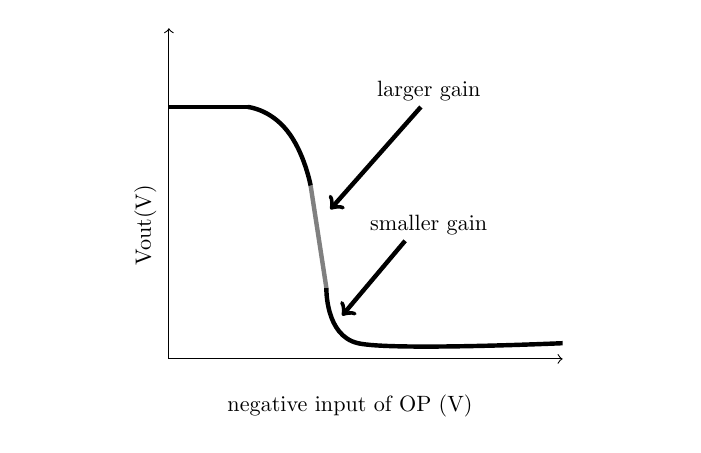
\begin{tikzpicture}
        \draw [black, ultra thick] plot coordinates { (0,4) (1,4) };
        \draw [black, ultra thick] plot [smooth, tension=1] coordinates { (1,4) (1.5,3.7) (1.8,3) };
        \draw [gray, ultra thick] plot [smooth, tension=1] coordinates { (1.8,3) (2,1.7) };
        \draw [black, ultra thick] plot [smooth, tension=0.5] coordinates { (2,1.7) (2.4,1) (5, 1) };

        \draw[->] (0, 0.8) -- (0, 5);
        \draw[->] (0, 0.8) -- (5, 0.8);
        \draw[->, ultra thick] (3.2, 4) -- (2.05,2.7);
        \draw[->, ultra thick] (3, 2.3) -- (2.2,1.35);
        \node[text width=5cm, scale=0.8, align=center] at (3.3, 2.5)
            {smaller gain};
        \node[text width=5cm, scale=0.8, align=center] at (3.3, 4.2)
            {larger gain};
        \node[text width=10cm, scale=0.8, align=center] at (2.3, 0.2)
            {negative input of OP (V)};
        \node[text width=5cm, scale=0.8, align=center, rotate=90] at (-0.3, 2.5)
            {Vout(V)};
    \end{tikzpicture}
    \caption{...}
    \label{fig:chip:line}
\end{figure}


\subsubsection*{Input Offset Voltage}
Another reason may be responsible for the low-current defect is the offset voltage at the input of the OP.

We examined the output voltage of TIA ($V_{TIA}$) of the Fig.\ref{fig:chip:IdIbiasVG} DC-sweep experiment.
It is shown in Fig.\ref{fig:chip:VTIA}.
Ideally, when feedback mechanism works well, $V_{TIA}$ should be equal to $V_{Ref}$(Fig.\ref{fig:chip:DCmode}).
However, the value of $V_{Ref}$ is $0.802 V$, which is smaller than $V_{TIA}$.
(This $V_{Ref}$ is connected to a constant voltage point inside the chip.
We know its value indirectly by measuring the drain voltage of nanowire since the drain of nanowire is kept to be same as $V_{Ref}$ by TIA.)
When the circuit works well, $V_{TIA}$ and $V_{Ref}$ is still different by $15m V$.
This voltage difference can result in an $150n A$ offset current flowing through TIA and into the nanowire device.
This offset current becomes remarkable when the $I_{bias}$ is less than $1\mu A$.

We suggest the reason that $V_{TIA}$ is large than $V_{Ref}$ is due to the offset voltage appearing at the input of the OP.
This speculation is reasonable through with respect to the layout, which will be discussed in the next section.

\begin{figure}[tbh!p]
    \centering
        \includegraphics[width=0.7\textwidth] {images/chapter6/gvt_0101Manual_VopiProblem.png}
    \caption{The $V_{TIA}$. The x-axis is the corresponding gate voltage.
                With the information from Fig.\ref{fig:chip:IdIbiasVG}, we found that the $V_{TIA}$ is not equal to $V_{Ref}$ no matter feedback mechanism works well or not.}
    \label{fig:chip:VTIA}
\end{figure}

Overall, the insufficient gain and the input offset may be the main reasons of the low-current defect.
Both of them relate to the OP block.
We then discuss these two reasons from the perspective of layout.

\subsection{The Design and Layout Problems of OP}
In the last section, me mentioned that the gain of OP is lower than we expected and there may exist an input offset voltage.
In this section, we will deduce that several layout and design flaws may be responsible for these two problems.

\begin{figure}[tbh!p]
    \centering
    \includegraphics[width=1\textwidth] {images/chapter6/OP_schematic.png}
    \caption{The left section is the schematics of the OP. The right section is a global circuit for generating the two global biasing voltage: $V_{bi}$, $V_{Ref}$.
                The Iin is an external current source.}
    \label{fig:chip:OPScem}
\end{figure}

\subsubsection{The Possible Reasons for Insufficient Gain}
The schematic presented in Fig.\ref{fig:chip:OPScem} contains two sections.
The left section is the body of the OP, while the right one is a global biasing circuit.




\section{Transient Measurement Mode}

\section{Dealing with the Device Variability Problem}



%==============================================================
\backmatter

% The following two commands are all you need in the
% initial runs of your .tex file to
% produce the bibliography for the citations in your paper.
{
\bibliographystyle{abbrv}
\bibliography{data/thesis}
}
% You must have a proper ".bib" file
%  and remember to run:
% latex bibtex latex latex
% to resolve all references

%==============================================================

\chapter*{\centerline{Acknowledgement}}



\end{document}
